\chapter{Literature Review}
\label{ch:litrev}

The following literature review first addresses current integration of 
repository modeling within systems analysis, followed by a discussion of the 
disposal system concepts and geologic host media under consideration 
domestically and internationally.  Finally, a review of analytical and 
computational models of radionuclide and thermal transport follow. 

\section{Repository Capabilities within Systems Analysis Tools}
\label{sec:SA_repos}

%%%%%%%%%%%%%%%%%%%%%%%%
% Systems Analysis Repository Capabilities
%%%%%%%%%%%%%%%%%%%%%%%% 
% The total system performance assessment is one type.Repository modules 
% incorporated into VISION and whatnot are another type.  Things to ask about 
% each of them include: % Which geologic media do they model?  How long do they take 
% to run?  Are they proprietary?  How well validated are they?  Do they include 
% any notion of repository capacity, dose, heat?  Are they capable of dealing 
% with waste of varying compositions?  Are therewasteform models?  Is there 
% radionuclide transport, source term estimate?  Heattransport?

%% This Section comes from 2011 CFP Narrative 3067, only lightly edited %%


Several computational fuel cycle simulation tools have been developed to inform 
calculations of fuel cycle metrics. This literature review focused on seven : 
\gls{NUWASTE} \cite{abkowitz_nuclear_2010},
\gls{DANESS} \cite{yacout_daness_2011,van_den_durpel_daness:_2006}, 
\gls{NFCSim} \cite{schneider_nfcsim_2004},
ORION \cite{gregg_orion_2011},
\gls{COSI} \cite{boucher_international_2010},
\gls{VISION} \cite{yacout_vision_2006, wilson_comparing_2011, 
radel_repository_2007, boucher_international_2010}, and
\gls{CAFCA} \cite{guerin_impact_2009}.

\subsection{Repository Performance Calculations}

Most current tools treat the waste disposal 
phase of fuel cycle analysis statically in post processing by reporting 
values such as mass, volumes, radiotoxicity, or heat production of accumulated 
\gls{SNF} and \gls{HLW}. Such tools 
(e.g.,
\gls{NUWASTE} \cite{abkowitz_nuclear_2010},
\gls{DANESS} \cite{yacout_daness_2011,van_den_durpel_daness:_2006}, 
\gls{NFCSim} \cite{schneider_nfcsim_2004}, and
ORION \cite{gregg_orion_2011}
) 
fail to address the impact of those waste streams on the performance of the 
geologic disposal system \cite{wilson_comparing_2011}.  Two tools, \gls{COSI} 
\cite{boucher_international_2010} and \gls{VISION} \cite{yacout_vision_2006, 
wilson_comparing_2011, radel_repository_2007, boucher_international_2010}, 
dynamically perform heat based capacity calculations.
However, those calculations are applicable only for specific 
repository concepts and cannot inform sensitivity to alternate geologic disposal 
system characteristics.  

\subsection{Detail}

A few sophisticated fuel cycle tools  (e.g.,
\gls{NUWASTE} \cite{abkowitz_nuclear_2010},
\gls{NFCSim} \cite{schneider_nfcsim_2004}, and 
\gls{COSI} \cite{boucher_international_2010}) have emphasized discrete material 
tracking and have demonstrated the improved flexibility of that strategy over more 
traditional flow sheet calculations. A few (e.g., 
\gls{NUWASTE} \cite{abkowitz_nuclear_2010} and
\gls{COSI} \cite{boucher_international_2010}
) utilize discrete material tracking to 
provide per-package metrics including heat generation and radiotoxicity. 


The number of isotopes distinctly tracked also varies among fuel cycle 
simulator tools. Some (e.g., 
\gls{COSI} \cite{boucher_international_2010},
\gls{DANESS} \cite{yacout_daness_2011,van_den_durpel_daness:_2006}, 
ORION \cite{gregg_orion_2011}, and
\gls{VISION} \cite{yacout_vision_2006, wilson_comparing_2011, radel_repository_2007, boucher_international_2010}
) are capable of tracking thousands or arbitrary numbers of isotopes. Others (e.g., 
\gls{NUWASTE} \cite{abkowitz_nuclear_2010}) track tens of isotopes, while still 
others neglect isotopic granularity (e.g., 
\gls{CAFCA} \cite{guerin_impact_2009}).

\subsection{Accessibility}

While these tools have contributed to analysis of fuel cycle effects on 
repository metrics, none address radionuclide contaminant transport in generic 
geologic media, and many (e.g.,
\gls{COSI} \cite{boucher_international_2010},
\gls{DANESS} \cite{yacout_daness_2011,van_den_durpel_daness:_2006}, 
ORION \cite{gregg_orion_2011},
\gls{NUWASTE} \cite{abkowitz_nuclear_2010}, and
\gls{VISION} \cite{yacout_vision_2006, wilson_comparing_2011, radel_repository_2007, boucher_international_2010}
) are too restrictively licensed for broad use and development. 


The current capabilities of these tools suggest that sensitivity of repository 
performance metrics to fuel cycle decisions can be calculated using a variety of 
methods that have yet to be explored. Based on the flexibility of discrete material 
tracking, power of dynamic modeling, and flexibility of open access the \Cyder 
tool has emphasized those strategies. Also, recognizing the need for a tool 
that analyzes repository performance for generic geologic settings, the \Cyder tool 
employs both thermal and contaminant transport capabilities.

\subsection{Repository Focused Fuel Cycle Analyses}

While top level fuel cycle system analyses fail to incorporate repository 
models, some repository focused fuel cycle sensitivity analyses have been conducted. 
Most domestic repository focused analyses have emphasized used fuel disposition and
waste management in the \glsreset{YMR}\gls{YMR}. These have been conducted by
Ahn \cite{ahn_environmental_2007}, 
Bauer \cite{bauer_geologic_2007}, 
Li \cite{li_examining_2007}, 
Piet \cite{piet_which_2007}, 
Radel \cite{radel_determination_2007}, 
Wigeland \cite{wigeland_criteria_2006,wigeland_separations_2006}, 
and others. With a focus on \gls{YMR} capacity benefit, 
repository performance metrics of interest for these analyses were heat, source 
term, and more global environmental impact metrics.  

The \gls{TSM} code, 
developed at \gls{OCRWM} is a very detailed model of the Yucca Mountain disposal 
system. It includes transportation issues and detailed emplacement timing and 
strategy models, but considers only the fuel cycle associated with the current  
U.S.  reactor fleet. Casks are modeled discretely and radionuclide and heat transport 
are modeled in great detail.  This level of detail results in a dramatically extended
run time making this model inappropriate for top level fuel cycle systems analysis. 
The \gls{TSM} model can only be run by its development team and runs a typical 
simulation, processing 70,000 MTHM, in 12-15 hours \cite{turner_discrete_2010}. 

The TSM framework is based on the commercial SimCAD platform. The simulation 
steps through times in 8 hour time steps during the waste cask transportation, 
processing and emplacement. This event based simulator is primarily focused on 
the operation stage of the Yucca Mountain repository, but is equipped with a 
thermal management model that informs waste package emplacement.

\section{Disposal Environment Concepts}

% To capture the broad distinctions, we'll model three geologic media
% and four concepts
% with flexible layouts
% and an array of available canonical subcomponents. 

% Certain things are true about the concepts we're considering
% reducing vs. oxidizing
% fractured vs. unfractured
% varying permeability
% varying depth
% varying layout


% We've looked at many international and domestic efforts
% They mostly involve closed, saturated, reducing concepts in granite, clay, and 
% salt media. Numerous tunnel emplacement types and repository layouts have been 
% considered and it's the goal of this work to capture the distinctions between 
% this option space.

A suite of three geologic media and four disposal concepts of interest were 
chosen to capture those found in the following review of 
international and domestic efforts. \Cyder has been developed to model granite, 
clay, and salt geologic environments with various layouts and an array of 
canonical engineered barrier component models.  

%The detailed \gls{GPAM} effort and 
%associated \gls{GDSM} tools were chosen to support the for this work will 
%support abstraction for these concepts and further comparison with \gls{ANDRA} 
%and RED-IMPACT results will provide further benchmarks for validation.  
Geologic disposal concepts that have been investigated internationally, with the 
exception of \gls{YMR}, can be characterized as enclosed concepts in saturated, 
reducing environments.  Saturated concepts are those located below the water 
table such that, in contrast to \gls{YMR}, the porosity within the rock matrix 
as well as fractures and other open spaces is suffused with water. An enclosed 
concept is one that neither relies on ventilation shafts nor an extended open 
period after waste emplacement.  In low permeability rock formations 
(clay/shale, granite, salt), an enclosed concept does not permit significant 
oxygen entry, typically resulting in chemically reducing environments.

Chemically reducing geologic environments are reducing insofar as they induce 
reduction of water flowing through them. That is, reduction and oxidation 
reactions in these environments proceed in such a way that electrons are 
donated to the water from the geologic medium. This attribute has the primary 
effect of slowing corrosion, dissolution, and  alteration rates in materials 
that are subject to degradation. A reducing disposal environment also lowers 
solubility limits and increases sorption of many actinide species. The dominant 
dose contributors in reducing environments are therefore the soluble, long 
lived fission and activation products such as $^{129}I$ and $^{79}Se$ 
\cite{oecd_nuclear_energy_agency_advanced_2006, von_lensa_red-impact_2008}.  
%Furthermore, rather 
%than being primarily kinetically limited, as in an oxidizing environment, 
%sorption behavior is primarily thermodynamically limited 
%\cite{nutt_personal_2011, schwartz_fundamentals_2004}. 

Various engineered barrier system components will also be modeled as a part of 
this effort.  Specifically, in order to cover the option space demonstrated by 
both domestic and international repository concepts, models must be developed 
which can interchangeably represent concrete, salt, and bentonite buffer and 
backfill options as well as waste package and waste form concepts which can be 
distinguished by their alteration, corrosion, and other degradation behaviors.


\subsection{Clay Disposal Environments}

Clays, including a range of claystones, shales, and argillites, have been 
investigated in Belgium, France, Japan, and Switzerland 
\cite{von_lensa_red-impact_2008} as well as the  \gls{US} 
\cite{clayton_generic_2011}. Due to low permeability and few fractures in clays, 
diffusion is the dominant transport mechanism. Additionally, clays tend to have 
high sorption capacity for cations, which reduces the mobility of contaminants 
present in clays as cations such as the lanthanides and americium 
\cite{higgo_clay_1987}.  A less attractive quality of clay is a low thermal 
limit around $100^{\circ}C$ temperature limit to prevent alteration 
\cite{hardin_generic_2011}.  Some characteristics of clay disposal concepts are 
given in Table \ref{tab:clay_tab}.   

%        File: clay_tab.tex
%     Created: Thu Aug 04 11:00 AM 2011 C
% Last Change: Thu Aug 04 11:00 AM 2011 C
%
\begin{table}[h!]
  \centering
  \footnotesize{
  \begin{tabular}{|l|l|l|l|}
    \multicolumn{4}{c}{\textbf{Clay Repository Features}}\\
    \hline
     Hydrology & Geochemistry & Design Concepts & Thermal Behavior \\ 
    \hline
    very low conductivity&reducing&&limit due to EDZ enlargement with heat\\
    high primary porosity (up to 0.5)&saline&&potentially 100C limit if bentonite buffer\\
    very low effective porosity&pH&no/bentonite/concrete backfill&\\
    slow water movement&saturated&horizontal, vertical, or room emplacement&\\
    diffusion dominates&&closed&\\
    &&<(-100m)&\\
    \hline
  \end{tabular}
  \caption[Clay Repository Features]{Clay geological repository 
  concept demonstrates certain dominant physical phenomena. }
  \label{tab:clay_tab}
  }
\end{table}




\subsubsection{Disposal System Components}

The French \gls{ANDRA}  analysis modeled borosilicate glass as well as ceramic 
oxide waste forms within carbon steel waste packages in combination with a bentonite 
buffer material and a crushed clay or shale backfill \cite{andra_argile:_2005}.
The Belgian reference concept focused on a highly plastic Boom Clay, which 
eventually completely seals around stainless steel, nickel, or titanium waste 
packages \cite{ondraf-niras_technical_2001}.  The Swiss concept modeled glass 
waste forms in stainless steel waste packages with a bentonite buffer and a 
bentonite and sand backfill
\cite{johnson_calculations_2002}. Each of these concepts considered 
horizontal emplacement in multiple-package emplacement drifts. 


\subsubsection{Hydrology}

In a clay disposal environment, exceptionally low interconnected porosity and 
very little fracturing result in a very low overall hydraulic conductivity and 
diffusion dominated water movement. 

\subsubsection{Geochemistry}

This environment is very reducing in both the near and far field, its salinity 
increases with depth, and its pH is expected to be near neutral. However, for 
some concepts incorporating cementitious backfill materials for protection 
of steel, the pH can become significantly alkaline, resulting in 
expedited alteration of glass waste forms, bentonite buffers, and the clay 
matrix \cite{andra_argile:_2005}.

%Clays tend to have higher sorption capacity for cations (what interesting 
%elements are cations?) \cite{bahr_private_2011}.
Radionuclides that are relatively highly mobile in a clay environment dominate 
potential long-term to the public from clay repository concepts.  Tor most fuel 
cycles, these include $^{129}I$, $^{79}Se$, and $^{36}Cl$ 
\cite{swift_applying_2010}. 

\subsubsection{Thermal Behavior}
\label{sec:claythermal}


Heat limits in clay are based on the domain of known behavior in clay and the 
tendency for bentonite fill material to lose its isolating properties with high 
temperatures \cite{andra_argile:_2005, pusch_alteration_1987}. 
The alteration of high smectite bentonite to non-expandable clays is a primary 
limitation for heat tolerance in the clay concept. The isolation characteristics 
of bentonite buffer materials are reduced after this alteration. The time 
integral of this phenomenon determines total bentonite alteration. While short 
bursts of heat might be allowable, because the bentonite will not alter 
immediately, the kinetic alteration into smectite clays is hastened by 
temperatures above approximately 100$^{\circ}C$\cite{pusch_alteration_1987}. 
Well understood behavior for argillaceous clay and bentonite buffer backfill
is conservatively assumed by the \gls{ANDRA} assessment to occur only under  
90$^{\circ}C$, which is effectively a limit at the waste package interface with 
the bentonite buffer material\cite{andra_argile:_2005} .
The \gls{NAGRA} Opalinus Clay assessment less conservatively 
uses a maximum heat limit in the bentonite buffer of $125^{\circ}C$
\cite{johnson_project_2002} .

%as with the waste packages in this geology.  

% 
% ``This low permeability of the Callovo-Oxfordian, linked to low hydraulic head 
% gradients on either side of the formation, controls slow vertical water flow 

The thermal conductivity of clay is also typically lower than 
$2[W\cdot m^{-1} \cdot K^{-1}]$. 
Accordingly, thermal loading constraints are more restrictive than in more 
conductive materials. 
In particular, Belgium (ref. 
\cite{ondraf-niras_technical_2001}) 
used values between 1.25 and 1.7 $[W\cdot m^{-1}\cdot K^{-1}]$,
France (ref. \cite{andra_argile:_2005}) used values between 1.9 and 2.7 
$[W\cdot m^{-1}\cdot K^{-1}]$, and Switzerland (ref. 
\cite{johnson_calculations_2002}) used 1.8 $[W\cdot m^{-1}\cdot K^{-1}]$.

% (Inset 3.5). The velocities of this water flow are fairly different in detail 
% because of the medium's pore structure. Moreover, some pores are not connected 
% and cannot take part in the water flow. A so-called kinematic porosity is 
% therefore defined, which is a fraction of total porosity, used macroscopically 
% to calculate mean water flow velocity in the direction of the hydraulic head 
% gradient. For the Callovo-Oxfordian, this kinematic porosity has been taken as 
% being the same as the fraction of free water in the rock, i.e. about 9 
%, corresponding to half the total porosity.  The very low permeability 
%determines average flow speeds within the layer (Darcy flux, inset 3.5) at 
%around 3 cm per 100,000 years, which corresponds to a water transfer velocity 
%of about 30 cm per 100,000 years, considering the kinematic porosity.  
%\cite{argile_geo_evo} 

% Water flow in a porous medium is dominated by darcy flow.  This would be a 
% great place to describe darcy's law! 

\subsection{Granite Disposal Environments}

Granite disposal concepts have been considered in Finland, France, Japan, 
Sweden, China,  Spain, the Czech Republic, South Korea, and Switzerland 
\cite{andra_granite:_2005, von_lensa_red-impact_2008} as well as the \gls{US} 
\cite{hardin_generic_2011}.

Attributes of granite that make it an attractive candidate geology for nuclear 
waste disposal include its very low porosity and permeability and high thermal 
conductivity. Fracturing in granite, however, has a negative effect on the 
isolation properties of the rock.
Some characteristics of granite disposal 
concepts are given in Table \ref{tab:granite_tab}.   

%        File: granite_tab.tex
%     Created: Thu Aug 04 11:00 AM 2011 C
% Last Change: Thu Aug 04 11:00 AM 2011 C
%
\begin{table}[h!]
  \centering
  \footnotesize{
  \begin{tabular}{|l|l|l|l|}
    \multicolumn{4}{c}{\textbf{Granite Repository Features}}\\
    \hline
    Hydrology & Geochemistry & Design Concepts & Thermal Behavior \\ 
    \hline
    Low porosity ($\sim 0.01$)&Reducing in Near Field&Single WP tunnels&Closed\\
    High Fracturation & Slightly Oxidizing in Far Field & Carbon-Steel \cite{andra_granite:_2005}or & Bentonite Limit $100^\circ C$\\
    Low permeability  &  Increasing saline with depth \cite{von_lensa_red-impact_2008} & Copper overpack&\\
    High Water Velocity& Cement causes alkalinity \cite{andra_granite:_2005}& Bentonite buffer &\\
    & Saturated or Unsaturated & Crushed granite backfill \cite{von_lensa_red-impact_2008}& \\
    &&$\sim100m$ deep&\\
    \hline
  \end{tabular}
  \caption[Granite Repository Features]{Granite repository 
  concepts demonstrate certain dominant physical phenomena.}
  \label{tab:granite_tab}
  }
\end{table}




\subsubsection{Disposal System Components}

The Swedish KBS-3 concept includes ceramic oxide spent fuel waste forms within a 
steel shell and copper waste package buffered by bentonite clay and backfilled 
with clay and sand and emplaced vertically in horizontal drifts 
\cite{ab_long-term_2006}.
A similar Czech Republic repository concept consists of 
borosilicate glass waste forms within a stainless steel Universal Canister waste 
package, vertically emplaced in horizontal drifts and with a bentonite buffer  
and backfilled with a clay and sand mixture.
The Spanish concept is almost exactly similar to 
these, except emplacement is horizontal within the horizontal repository drifts
\cite{ von_lensa_red-impact_2008}.


%Japanese studies investigated numerous layouts. . .  Finland china south korea switzerland. 
%UFD <+more details?+>


\subsubsection{Hydrology}

In the granite disposal environment, a low porosity is combined with 
higher expected water velocity (relative to other repository concepts in this 
work) and significant fracturing. The overall 
granite hydraulic conductivity is still typically low
\cite{schwartz_fundamentals_2004, 
hardin_generic_2011}. Within this environment, the  
water behavior in the far field must be modeled as both diffusive and advective.

\subsubsection{Geochemistry}

This environment is very reducing in the near field and slightly less so in the 
near surface far field due to far field fracturing in the granite near the 
surface. Most importantly, this results in higher actinide solubilities in that 
region. Salinity in the granite environment increases monotonically with depth. 
At a typical concept depth of 500m, the repository is therefore expected to be 
in a location of high salinity, an indicator of historically low fluid flow but 
resulting in increased corrosion rates and for some radionuclides, changed 
solubilities \cite{andra_granite:_2005}.  It is expected that the pH will be 
near neutral in this environment except with  the introduction of concretes, 
due to which the pH becomes significantly alkaline, resulting in more rapid 
alteration of bentonite buffers. 

The relatively fast advective pathways in fractures have the effect of 
increasing the importance of $^{234}U$ in the initial waste stream. While 
$^{234}U$ and its decay daughter $^{230}Th$ are not very mobile in a reducing 
environment, their subsequent decay daughter $^{226}Ra$ is highly mobile.  
$^{226}Ra$ is therefore a dominant dose contributor in granite 
\cite{swift_applying_2010}, while in many other geologies, the 1601 year half 
life of $^{226}Ra$ is too short for a significant quantity to traverse the 
diffusive pathway.

\subsubsection{Thermal Behavior}
\label{subsec:granitethermal}
In the absence of a bentonite limitation (i.e., concepts with non-bentonite 
buffers), a thermal limit within the granite itself is greater than 
$200^{\circ}C$, limited by the increased risk of micro-cracking.
Mechanical stresses and strains in the matrix due to heating at this 
level were analyzed by \gls{ANDRA} and shown to have a negligible effect of 
flow behavior in granite. Similarly, thermo-hydraulic effects due to thermally
induced fluid density changes are expected to be slight 
\cite{andra_granite:_2005}.
Similarly, for reasons of buffer isolation integrity, the Czech and Spanish
granite disposal concepts both maintained a thermal limit at the waste package
interface with the buffer of $100^{\circ}C$.  \cite{von_lensa_red-impact_2008}

This relatively high resistance to heat  induced mechanical failure is due to the 
high thermal conductivity of granite, which is typically found to be between 
2.4 and 4 $[W\cdot m^{-1}\cdot K^{-1}]$.  In particular Sweden (ref. 
\cite{ab_long-term_2006}) used 3.4 - 4 $[W\cdot m^{-1}\cdot K^{-1}]$  and 2.45 
- 2.9 $[W\cdot m^{-1}\cdot K^{-1}]$,  France (ref.  \cite{andra_argile:_2005}) 
used 2.4 - 3.8 $[W\cdot m^{-1}\cdot K^{-1}]$, and  Finland (ref. 
\cite{posiva_interim_2010}) used 2.3 - 3.2 $[W\cdot m^{-1}\cdot K^{-1}]$.

The effective thermal limit for granite disposal concepts, however, is usually 
related to the bentonite limit, which is similar to the bentonite limits of clay 
concepts discussed in Section \ref{sec:claythermal}.

\subsection{Salt Disposal Environments}

Salt disposal concepts have been investigated in Germany and demonstrated for 
non-heat-generating waste at the \gls{WIPP} facility in the US. Salt 
demonstrates many attractive properties including ease of mining, creep behavior 
over time, which is expedited by heat, low permeability, and a high thermal 
conductivity, which affords a high temperature limit near $200^{\circ}C$ 
\cite{hardin_generic_2011}.
Some characteristics of salt disposal 
concepts are given in Table \ref{tab:salt_tab}.   

%        File: salt_tab.tex
%     Created: Thu Aug 04 11:00 AM 2011 C
% Last Change: Thu Aug 04 11:00 AM 2011 C
%
\begin{table}[h!]
  \centering
  \footnotesize{
  \begin{tabular}{|l|l|l|l|}
    \multicolumn{4}{c}{\textbf{Salt Repository Features}}\\
    \hline
    Hydrology & Geochemistry & Design Concepts & Thermal Behavior \\ 
    \hline
    Dry Waste Package & Reducing in Near Field & Alcove Emplacement & $180^\circ C$ limit \cite{von_lensa_red-impact_2008} \\
    Dry Backfill &Far Field Slightly Oxidizing &Crushed Salt Backfill & Heat induced creep sealing\\
    Saturated Far Field& Very saline brines  &$\sim100m$deep & Closed \\
    Very low permeability &  & Multiple Packages &limited data\\
    Brine pockets in far field&&Breached only from intrusion&\\
    \hline
  \end{tabular}
  \caption[Salt Repository Features]{Salt geological repository 
  concept demonstrates certain dominant physical phenomena. }
  \label{tab:salt_tab}
  }
\end{table}


% The heat limit may be because the creep is too fast. 




\subsubsection{Disposal System Components}

German and United States salt concepts include drifts or alcoves, respectively, 
in which waste packages are placed. The space is then backfilled with crushed 
salt \cite{von_lensa_red-impact_2008}.  The consolidation properties of the 
backfill and salt are of great isolation importance. The infinitesimally small 
hydraulic conductivity of consolidated rock salt has the effect of nullifying 
the possibility of any releases without a disruption scenario 
\cite{brewitz_long-term_2002}.


\subsubsection{Hydrology}

In a rock salt or salt dome disposal environment, a very low porosity combined 
with negligible water velocity and effectively no fracturing results in a 
salt hydraulic conductivity that is exceptionally low. Within this environment,   
extraordinarily slow diffusive speed out of the repository dominates the 
isolation behavior. Candidate salt formations are remarkably uniform and their 
accessible porosity is near negligible, so almost no water movement is expected to 
occur. 

\subsubsection{Geochemistry}

This environment is very reducing in the near field and slightly less so in 
the far field \cite{clayton_generic_2011}. Very high salinity
expedites corrosive processes, but the engineered barrier system 
is of limited importance in this concept in which the diffusive geologic salt barrier 
dominates isolation integrity.  It is expected that the pH will be near
neutral in this environment \cite{von_lensa_red-impact_2008, clayton_generic_2011}.

\subsubsection{Thermal Behavior}
\label{subsec:saltthermal}

Response of a salt repository to heat has a significant
mechanical component. Bulk heating of a salt repository matrix causes
coalescing  of the salt surrounding the heat source. In the case of a nuclear
waste repository, this phenomenon increases isolation capability of the salt. A
heat limit, then, is difficult to characterize, but evolution of the heat in a
salt environment is of great importance to radionuclide transport modeling. 

The German salt repository concept maintains a $180^\circ C$ temperature limit. 
The technical basis for this limit has to do with the concern that at
temperatures above $220^\circ C$ differential densities in the salt formation 
may drive the movement of brine inclusions and potentially facilitating radionuclide transport 
\cite{von_lensa_red-impact_2008, brewitz_long-term_2002, lee_preliminary_2012}. 

Notably, the crushed salt backfill in most concepts has low conductivity, which 
increases the sensitivity of rock salt temperature on emplaced package 
temperature. However, as the crushed salt coalesces with heat over time, its 
thermal conductivity increases to approach that of intact salt. Further 
investigation toward a comprehensive model of the thermal behavior of dry salt 
has been recommended both domestically and internationally 
\cite{carter_generic_2011}. 

%The behavior of moisture in a salt repository under high heat is also not well 
%characterized . Though it is clear that the salt will creep and coalesce with 
%increased temperature, the potential generation of brines within the salt at 
%high heat is a pertinent issue for salt disposal characterization. 

\subsection{Deep Borehole Disposal Environments}

Deep Borehole disposal system concepts are being evaluated in the UK, 
Sweden and the United States \cite{von_lensa_red-impact_2008, 
clayton_generic_2011}. Attributes of this concept that are 
favorable for waste isolation include the stability of the crystalline 
basement rock in which the borehole emplacement would occur and the elongated
diffusion path length for release. The potential technical difficulty of well 
controlled emplacement at great depth is an unfavorable attribute, however 
\cite{hardin_generic_2011}.  Some characteristics of deep borehole disposal 
concepts are given in Table \ref{tab:borehole_tab}.   

%        File: borehole_tab.tex
%     Created: Thu Aug 04 11:00 AM 2011 C
% Last Change: Thu Aug 04 11:00 AM 2011 C
%
\begin{table}[h!]
  \centering
  \footnotesize{
  \begin{tabularx}{\textwidth}{|X|X|X|X|}
    \multicolumn{4}{c}{\textbf{Borehole Repository Features}}\\
    \hline
    Hydrology & Geochemistry & Design Concepts & Thermal Behavior \\ 
    \hline
    Crystalline rock&Reducing at depth& $\sim5km$ deep & cracking unimportant\\
    Low porosity ($\sim 0.01$)&Less Reducing at surface& disposal in lower 2km &may affect flow\\
    Limited fracturing at depth&limited solubility &1km betonite seal & high conductivity\\
    Rock Permeability ($\sim 10^{-19}$) &enhanced sorption &bentonite grout &high density\\
    EBS Permeability ($\sim 10^{-16}$) &high salinity&bentonite plugs&\\
    Very Limited Upward Flow&&400 packages per borehole&\\
    &saturated&closed&\\
    \hline
  \end{tabularx}
  \caption[Borehole repository features.]{Borehole geological repository 
  concept demonstrates certaindominant physical phenomena. }
  \label{tab:borehole_tab}
  }
\end{table}


\subsubsection{Disposal System Components}

In deep borehole concepts, many types of  waste form and waste package material 
are emplaced at great depths, typically between 2 and 5 km 
\cite{hardin_generic_2011, clayton_generic_2011}
in a crystalline rock such as granite basement rock. In each borehole, hundreds
of canisters are stacked vertically in the deepest section. In some concepts, 
dense bentonite plugs are stacked between the packages. Above the packages, 
swelling bentonite clay, asphalt and concrete provide a seal for the upper few 
kilometers \cite{clayton_generic_2011}. 

\subsubsection{Hydrology}

In the deep borehole crystalline basement rock disposal environment, low porosity
combined with only minor fracturing results in an overall 
hydraulic conductivity which is very low. Thermally driven, upward water 
velocity is the primary driver for solute movement along the 2-5
kilometer diffusive path to the surface where fresh water aquifers may exist
\cite{clayton_generic_2011}.
Without the introduction of a fast pathway (e.g., an intersecting fracture or 
human intrusion) the length of the diffusive pathway has the effect of making the 
engineered barrier component choices irrelevant since no known engineered 
barrier choice can be expected to outlast the timescale of the diffusive pathway.

\subsubsection{Geochemistry}

This environment is very reducing in the near field and less in the very 
far field near the earth's surface. The very high salinity of this environment
is due to its depth indicates historically low flow. While this increases 
corrosion rates of engineered barriers, the isolation worth of this concept 
does not depend significantly on the engineered barrier components, relying 
instead on the diffusion path length.  


\subsubsection{Thermal Behavior}
\label{subsec:boreholethermal}

Since the crystalline basement rock in which deep borehole concepts are 
envisioned is typically granite, the thermal behavior of the deep borehole 
environment is exactly similar to the granite case, except the bentonite buffer 
limitation is no longer applicable.  Also, the $200^{\circ}C$ limitation in 
order to avoid microfissures could  be shown to be irrelevant in light of the 
great distance to the surface. That is, even if the damage zone in the vicinity 
of the emplaced waste packages is enlarged significantly by high heat load, 
the kilometers of diffusion length to the surface will still dominate the 
isolation behavior of the repository. 


%%%%%%%%%%%%%%%%%%%%%%%%%%%%%%%%%%%%%% 

\section{Analytical Models of Radionuclide Transport} \label{sec:analytical_nuc}

%%%%%%%%%%%%%%%% Analytical Radionuclide Transport %%%%%%%%%%%%%%%%%%%%%%%%

Models of radionuclide contaminant transport address radionuclide transport 
through some or all of the release pathway made up of waste forms, waste packages, 
engineered barrier systems, and geologic media. A model of transport through 
the repository typically incorporates radionuclide release via waste 
form degradation, waste package failure, then advective and diffusive 
transport through the engineered barrier system and geologic medium. Some models also 
incorporate advective fast pathways introduced by tectonic events or human 
intrusions.

\subsection{Waste Form Release Models}

Radionuclide release, the mass transfer of a radionuclide from its 
waste form into surrounding water, 
from various possible waste form types will be dominated by 
an array of degradation, alteration, and dissolution phenomena. 
Some phenomena dominating the release from canonical waste forms such as  \gls{CSNF}, 
\gls{DSNF}, and borosilicate glasses are listed in Table \ref{tab:wf}.

%%%%%%%%%%%%%%%%%%%%%%%%%%%%%%%%%%%%%%%%%%%%%%%%%%%%%%%%%%%%%%%%%%%%%%%
%        File: litrev/wf_tab.tex
%     Created: Fri Aug 05 09:00 AM 2011 C
% Last Change: Fri Aug 05 09:00 AM 2011 C
%
\begin{table}[h!]
  \centering
  \footnotesize{
  \begin{tabular}{|l|l|c|c|}
    \multicolumn{4}{c}{\textbf{Waste Form Types}}\\
    \hline
    WF Type & SubTypes & Contents & Release Drivers  \\
    \hline
    \hline
    Once Through & \gls{CSNF} Ceramic Oxide & Nominal Burnup UOx \& MOX & redox reactions \\
                 & \gls{CSNF} Ceramic Oxide & High Burnup  & redox reactions, heat  \\
                 & \gls{HTGR} TRISO Graphite & High Burnup & graphite reactions\\
                 & \gls{DSNF} Metal  & High Burnup N Reactor Fuel & metal reactions,  heat\\
                 & \gls{DSNF} Carbides  & Fast Reactor Fuels & carbide reactions,  heat\\
                 & \gls{DSNF} Ceramic Oxides  & Research Reactor Fuels & redox reactions,  heat\\
    \hline
    Borosilicate Glass & Current & \glspl{MA} Cs/Sr & heat, glass alteration \\
                       & Future & Mo, no \gls{MA} no Cs/Sr & glass alteration  \\
    \hline
    Glass Ceramic & Glass Bonded Sodalite & Echem processed oxide fuels & ceramic, redox, glass reactions  \\
    \hline
    Metal Alloy & From Echem & Cladding, noble metals & metal reactions, heat \\
                & From Aqueous & undissolved solids, transition metals & metal reactions, heat  \\
    \hline
    Advance Ceramic &  & volatized iodine  & ceramic reactions, redox \\
    \hline
    Salt  & Cementitious Sodium  & separated streams  & alkaline reactions, dissolution \\
    \hline
  \end{tabular}
  \caption[Waste Form Types]{An array of waste forms developed for nuclear 
  wastes will have an array of dominant release 
  mechanisms.\cite{blink_disposal_2010}}
  \label{tab:wf}
  }
\end{table}



%%%%%%%%%%%%%%%%%%%%%%%%%%%%%%%%%%%%%%%%%%%%%%%%%%%%%%%%%%%%%%%%%%%%%%%

\subsubsection{Degradation Rates}
An initial breach of the primary barrier, which exposes the waste form to water, 
typically triggers degradation of the waste form \cite{bracke_safety_2008}.  
Degradation behaviors depend strongly water chemistry, but primarily on material 
properties of the waste form.  In the absence of detailed knowledge about long 
term waste form material behavior, however, waste form degradation can be 
modeled as a purely rate based model,

\begin{align}
  V_i(t) &= V_i(0)\left(1 - \int_0^t f(\cdots)dt\right)\\
         &= \mbox{intact waste form volume }[m^3]\nonumber\\
  \label{wfdegrate}
\end{align}

In the case of saturated repository concepts, degradation is often modeled to 
begin immediately at emplacement \cite{hedin_integrated_2002}. However, in 
models of unsaturated media \cite{ahn_environmental_2004, 
ahn_environmental_2007} , the waste form may not come into contact with water 
immediately, and therefore degradation will not begin until the onset of water 
contact,

\begin{align}
  V_i(t) &= V_i(0)\left(1 - \int_0^t f(\cdots)H(t-t_{wpf})dt\right).
  \intertext{where}
  t_{wpf} &=\mbox{time of waste package failure}\nonumber\\
  H(t-t_{wpf}) & = \mbox{Heaviside step function}\nonumber\\
      & = \begin{cases}
        0  & t<t_{wpf}\\
        1 & t\ge t_{wpf}
      \end{cases}
  \label{wfdegrate}
\end{align}


Importantly, the rate is often assumed to be slower in reducing environments than 
oxidizing ones\cite{swift_applying_2010}.

In either case, radionuclide release is often modeled as congruent with the 
degradation of the waste matrix. That is, release is modeled as unimpeded by 
sorption or solubility and becomes available according to the fractional 
degradation rate until the waste form is completely degraded 
\cite{ahn_environmental_2004, ahn_environmental_2007}.

If congruent release neglects transport retarding factors such as solubility 
limitation, it is most appropriate when applied to highly soluble radionuclides. 
In \cite{ahn_environmental_2004, ahn_environmental_2007} the transport of highly 
soluble radionuclides (those with high solubility limits) are modeled as 
infinitely soluble in this way. In an oxidizing environment, radionuclides of 
this type include most of the fission products, but not the actinides. 

\subsubsection{Solubility Limitation}

In order to account for solubility limitation, a threshold of elemental 
dissolved concentration, the reduced mobility of radionuclides with lower 
solubilities can be modeled \cite{hedin_integrated_2002} as a reduction in the 
amount of solute available for transport. For radionuclides with low 
solubility, the mass fraction released from the waste matrix is constrained to 
less than the solubility limit such that 

\begin{align} 
  m_{i}(t)&\le V(t)C_{sol, i}\label{sol_lim}
  \intertext{where}
  m_{i} &= \mbox{ mass of isotope i in volume }V [kg]\nonumber\\
  V &= \mbox{ a distinct volume of fluid } [m^3]\nonumber\\
  C_{sol, i} &= \mbox{ the maximum concentration of i } [kg\cdot m^{-3}].\nonumber
\end{align}

That is, the mass $m_{1i}$ in $[kg]$ of a radionuclide $i$ dissolved into the waste package
void volume $V_1$ in $[m^3]$, at a time t, is limited by the solubility limit, 
the maximum concentration, $C_{sol}$ in $[kg/m^3]$ at which that radionuclide is 
soluble \cite{hedin_integrated_2002}.

In the Ahn models, radionuclides with lower solubility limits are modeled with
a solubility limited release model.  Solubility values are assumed from TSPA
for this model, and elements with a solubility of less than $~5\times 10^{-2}
[mol/m^3]$ are taken to be
`low.' Elements in this `low' category include Zr, Nb, Sn and some toxic actinides 
such as Th and Ra for an oxidizing, unsaturated environment similar to \gls{YMR}.
It should be noted that in a reducing environment, the actinides are not as mobile, 
and the high and low solubility radionuclides will differ from this model.
This model suggests that dissolution of radionuclides into the water 
is dominated by diffusion, which is largely dependent upon the concentration 
gradient between the waste matrix and the water. The mass balance driving 
radionuclide release takes the form:

\begin{equation}
 \dot{m_i}=8\theta D_eS_iL\sqrt{\frac{vr_0}{\pi D_e}}
\end{equation} 

where $\theta$, v, $r_0$, and L are the geometric and
hydrologic factors porosity, water velocity, waste package radius, and waste
package length, respectively. $D_e$ is the effective diffusion coefficient
($m^2/yr$)  and $S_i$ is the solubility ($kg/m^3$) of isotope $i$.

\subsubsection{Flow Assumptions}

Water heavily affects the waste form degradation rate and is treated differently 
in various models. While some (`flowthrough models') assume water moves through 
the waste packages at a constant volumetric rate. Ahn 
\cite{ahn_environmental_2007}, for example models the water flow beginning at one 
waste package and travelling through the matrix and buffer space to the next 
waste package, contacting each waste package consecutively and then flowing on 
into the near field. In this way, the water is increasingly contaminated as its 
path through the waste packages proceeds.  Others adopt assumptions 
incorporating weather based predictions of hydrologic activity 
\cite{ahn_environmental_2007}.  

%%%%

\subsection{Waste Package Failure Models}

Waste package failure modes vary between models. Many analytic models of 
canister failure incorporate their own hydrologic approximations of
canister degradation or make simpler assumptions of immediate waste canister 
failure in order to focus on degradation and radionuclide release. 

Waste package failure depends on near field environmental factors such as decay 
heat and water chemistry.  
The radionuclide release rate from a waste 
package depends on the character of the waste form matrix and water flow as 
well as elemental solubility, sorption, and diffusion. 


Waste package failure can, in general, be represented with an expression of the 
number of failed waste packages failing per unit time, $n_F$. This is a simple 
product between the initial number of waste packages, $N$, and the rate, $f$, of 
failure

\begin{align}
  n_F = N\cdot f().
  \label{rate}
\end{align}

Some current common models addressed in this literature review appear in Table 
\ref{tab:wpfail}.

%%%%%%%%%%%%%%%%%%%%%%%%%%%%%%%%%%%%%% 
%%%%% WP Failure Modes Table %%%%%%%%%
%%%%%%%%%%%%%%%%%%%%%%%%%%%%%%%%%%%%%% 
\begin{table}[h!]
\centering
\footnotesize{
\begin{tabular}[h!bt]{|l|r|r|r|}
  \multicolumn{4}{c}{\textbf{Current Waste Package Failure Models}}\\
  \hline
  Model&WP Failure Mode&Waste Form&Details\\
  \hline
  TSPA&EBSFAIL&&$300,000$ years\\
  \hline
  Ahn 2003&Instantaneous Failure&Borosilicate Glass&$t=0$\\
  \hline
  Ahn 2007& &CSNF $UO_2$ matrix &$T_f=75,000$ years\\
  & &Borosilicate Glass &$T_f=75,000$ years\\
  & & Naval $UO_2$ matrix &$T_f=75,000$ years\\
  \hline
  Li&EBSFAIL&&$300,000$ years\\
  \hline
  Hedin 2003& Instantaneous & Copper KBS-3 Concept & $t_{delay} = 300$ years \\
  \hline
\end{tabular}
\label{tab:wpfail}
\caption[Current WP Failure Models]{The above represent current methods by which waste packeage 
failure rates are modeled.}
}
\end{table}

%%%%%%%%%%%%%%%%%%%%%%%%%%%%%%%%%%%%%%


\subsubsection{Physical Model}

When enough data exists, the waste package failure rate $f$ can
be represented more realistically by fractional destruction according to 
experimentally observed corrosion and dissolution rate functions.  However, this 
can be complicated to model even if the data exists. In particular, the 
corrosion rate will depend on the chosen material as well as hydrologic and 
thermal conditions. Specifically, corrosion rates for the same material are very 
different under dry oxidizing conditions and wet reducing conditions. 

The rate $f$ of package  failure in this case will be a function of time $t$, 
temperature $T$, and other physical parameters.

\begin{align}
  f() = N\cdot f(t,T,\cdots).
  \label{rate}
\end{align}

\subsubsection{Degradation Rate Based}
Rather than a discrete model, in which barriers fail completely at a collective 
rate, a fractional degradation rate per barrier can be used. For this type of 
model, the intact volume decreases at a fractional rate,

\begin{align}
  V_i(t) &= V_i(0)(1 - \int_0^t f(\cdots)dt)
  \intertext{which, for a constant rate, becomes}
  V_i(t) &= V_i(0)(1 - t).
  \label{wfdegrate}
\end{align}


\subsubsection{Probabilistic}

When a probability distribution of waste package failure is available, perhaps 
from extrapolated empirical observations, the discrete waste packages can be 
modeled to fail according to that distribution.  For example, if the expected 
lifetime of a waste package is some known $t_F$, a Gaussian distribution around 
$t_F$ would provide a probability density function for waste package failures 
per time step, $f(t)$,

\begin{align}
  f()=f(t).
  \label{probabilistic}
\end{align}

Expressed with a cumulative distribution function $F(t)$ rather than the
probability distribution function, equation \eqref{rate} becomes 


\begin{align}
  \sum_{t=0}^{t=t}n_F=N\cdot F(t).
  \label{cdf}
\end{align}


A particularly appropriate probability distribution for use in the case of failed 
engineered barriers is the Weibull distribution, which has a flexible shape 
capable of modeling a range of failure rates and can provide reasonably 
accurate predictions of failure based on small empirical data sets 
\cite{murthy_weibull_2004}. The Weibull distribution is expressed as

\begin{align}
  f(t,\lambda,k) =  \begin{cases}
    \frac{k}{\lambda}\left(\frac{t}{\lambda}\right)^{k-1}e^{-(t/\lambda)^{k}} & 
    t\geq0 ,\\
    0 & t<0 .\end{cases}
  \label{weibullpdf}
\end{align}


In this expression, $k$ is a shape parameter and $\lambda$ is a scale
parameter. The time to failure, $t$ in the Weibull distribution gives a 
distribution for which the failure rate is proportional to a power of time 
\cite{papoulis_probability_2002}. Its complementary cumulative distribution
function is 
\begin{align}
  F(t,\lambda,k) = 1-e^{-(t/\lambda)^k}.
  \label{weibullcdf}
\end{align}
For $k<1$, the rate of failure will decrease over time, while for a value of 
$k>1$, the rate increases over time, appropriate for the aging process of 
materials  \cite{papoulis_probability_2002}.



\subsubsection{Instantaneous}

The instantaneous case is a special case of the probabilistic situation.
Specifically, the probability density function is clearly just the Dirac 
delta function, with $n_F$ being the number of failed waste packages per 
unit time, $N$ being the total number of waste packages, and $t_F$ being 
the time to failure,

\begin{align}
  f()= \delta(t-t_F).
  \label{instantaneous}
\end{align}


The Hedin model of waste package failure is effectively instantaneous, but
limited by a release resistance coefficient. The release is assumed  to occur
through a hole in the waste canister that exists throughout the simulation, and
the resistance coefficient limiting flow through the hole represents the
magnitude of the canister flaw in combination with the buffer-geosphere
interface\cite{hedin_integrated_2002}.  Other models also use an instantaneous 
waste package failure mode for all waste  packages simultaneously, in which 
failure occurs either at the onset of the simulation or at some distinct time 
during the simulation. 


%%%%


\subsection{Radionuclide Transport Through Secondary Engineered Barriers}

When the waste package is breached and radionuclides are released from the waste 
form, radionuclides are transported through the secondary engineered barrier, 
which includes the buffer, backfill, and tunnel wall. After transport through 
the secondary \gls{EBS}, radionuclides reach the geologic medium. 

Diffusive and advective transport occur in the barrier matrix both before and 
after degradation.  The same models of waste package failure (instantaneous, 
rate based, and probabilistic) can be applied to secondary engineered barriers 
(i.e., buffer materials). While concretes are expected to degrade over time, 
bentonite buffers are quite stable in a reducing environment and help to keep 
the environment reducing. Furthermore, if preserved by a low heat environment, 
plastically deforming bentonite clays tend to swell over time and exhibit 
increased isolating behavior.  

Before degradation, transport is primarily diffusive.  Thereafter, transport can 
become advective due to cracking.  Radionuclide transport through the \gls{EBS} 
and host rock is driven by diffusion as well as advection. Radionuclide 
transport is retarded by sorption, limited by solubility, and possibly enhanced 
by colloidal mobility \cite{bracke_safety_2008}. 


%%%%

\subsection{Hydrologic Transport}

Transport through the geosphere in clay, shale, granite,
and salt can largely be characterized as solute transport in permeable porous 
media. While clay, shale and salt do not exhibit significant fracturing and can 
often be modeled as homogeneous, granite is  characterized as a fractured 
permeable porous media.  Solute transport in both fractured and homogeneous 
permeable porous media has both porous and fracture flow paths and involves
advection, hydraulic dispersion, and diffusion phenomena. 

Advection is transport driven by bulk water velocity, diffusion is the result of 
Brownian motion across concentration gradients, and hydraulic dispersion is 
transport resulting from heterogeneities in the water velocity field.  
Fundamentally, the effect of these flows on mass transport through a 
representative control volume is captured by the conceptual expression 

\begin{align}
  \mbox{In} - \mbox{Out} &= \mbox{Change in Storage}
  \label{inout}
\end{align} 

% Solute Transport in permeable porous media 

% advection - transport at the velocity of water flow 

% hydraulic dispersion - transport due to anisotropies in the water 

% velocity field. It depends on concentration of solute, darcy 

% velocity, and dispersivity.  

% diffusion - is from random brownian motion, tends to homogenize 
% concentration field.  %

Rearranging \ref{inout} and defining incoming and outflowing fluxes in a control  
volume,  solute transport in a permeable medium of homogeneous porosity can be
written (as in Schwartz and Zhang \cite{schwartz_fundamentals_2004})

\begin{align} 
  \frac{\partial \theta C}{\partial t} & = - \nabla \cdot  (F_c + F_{dc} + F_d) + m 
  \label{solperm}
  \intertext{where} 
  \displaybreak[0]
  \theta &= \mbox{solute accessible porosity } [\%]\nonumber\\
  C &= \mbox{ concentration } [kg \cdot m^{-3}]\nonumber\\ 
  t &= \mbox{ time } [s]\nonumber\\ 
  F_c &= \mbox{ advective flow } [kg \cdot m^{-2}\cdot s^{-1}]\nonumber\\
  &= \theta vC \nonumber \\
  \displaybreak[0]
  F_{dc} &= \mbox{ dispersive flow } [kg \cdot m^{-2}\cdot s^{-1}]\nonumber\\ 
  &= \alpha \theta v \nabla C  \nonumber\\ 
  \displaybreak[0]
  F_d &= \mbox{ diffusive flow } [kg \cdot m^{-2}\cdot s^{-1}]\nonumber\\
  &= \theta D_e \nabla C\nonumber\\
  \displaybreak[0]
  m &= \mbox{ solute source } [kg \cdot m^{-3}\cdot s^{-1}].\nonumber
  \displaybreak[0]
  \intertext{In the expressions above,} 
  v &= \mbox{ advective velocity } [m\cdot s^{-1}] \nonumber\\
  \alpha &= \mbox{ dispersivity } [m]\nonumber\\
  D_e &= \mbox{ effective diffusion coefficient } [m^2\cdot s^{-1}]\nonumber
  \displaybreak[0]
  \intertext{and} 
  \theta\cdot v &= \mbox{ Darcy flux } [m\cdot s^{-1}].
\end{align} 

The method by which the dominant solute transport regime (diffusive or advective)
is determined for a particular porous medium is by use of the dimensionless
Peclet number, 

\begin{align} 
  Pe &= \frac{\theta vL}{\alpha \theta v + D_e},\\
  &= \frac{\mbox{advective rate}}{\mbox{diffusive rate}}\nonumber
  \intertext{where} 
  L &= \mbox{ transport distance } [m].\nonumber
\end{align}

For a high $Pe$ number, advection is the dominant transport regime, while 
diffusive or dispersive transport dominates for a low $Pe$ number. If 
one of these terms can be neglected, the solution is simplified. 

Otherwise, the analytical expression in equation \eqref{solperm} will be the 
foundation of simplification by regression analyses for the radionuclide transport 
interface between components of the repository system model representing permeable 
porous media.  

It is customary to define the combination of molecular diffusion and mechanical
mixing as the dispersion tensor, $D$,  

\begin{align}
  D = \alpha v + D_e
  \label{dispersion}
\end{align}

such that the mass conservation equation becomes:

\begin{align}
  \nabla \left( \theta D\nabla C \right) - \nabla \left( \theta v \right) &= \frac{\partial(\theta C)}{\partial t}
  \label{massbal} 
  \end{align}

Sorption includes both absorption and adsorption. Absorption is the 
incorporation of a substance of one state into another of a different state.
Adsorption is the interaction of a dissolved species with a surface that
removes that species from the dissolving medium models. During sorption, 
contaminants are removed from the water and taken up by the 
walls of pores or fractures in the rock matrix.  The process that is the reverse 
of sorption is desorption in which the 
contaminant is returned to the pore or fracture fluid from the matrix
\cite{ahn_mass_1988} . Reversible sorption is typically expressed in terms 
the mass of a radionuclide sorbed into the rock and the mass left in solution. 
Sorption is a sensitive function of the redox state of the environment. Adding 
sorption to equation \eqref{massbal}, by accounting for a change in mass 
storage,

\begin{align}
  \nabla \left( \theta D\nabla C \right) - \nabla \left( \theta v \right)  &= 
  \frac{\partial(\theta C)}{\partial t}  + \frac{\partial(s\rho_b)}{\partial t} 
  \label{withsorption} 
  \intertext{where}
  s &= \mbox{sorbed phase concentration}\nonumber\\
  \rho_b &= \mbox{ bulk (dry) density }[kg/m^3].\nonumber
\end{align}

If sorption is approximated as a linear equilibrium, reversible reaction,

\begin{align}
s &= K_dC\\
\intertext{where}
K_d &= \mbox{ the distribution coefficient }[],\nonumber
\end{align}
then equation \eqref{withsorption} can be rewritten in terms of the so-called 
retardation factor,

\begin{align}
  \nabla \left( \theta D\nabla C \right) - \nabla \left( \theta v \right)  &= R_f\frac{\partial \theta C}{\partial t} 
  \label{withsorptionrf} 
  \intertext{where}
  R_f &= \mbox{retardation factor}\nonumber\\
   &= 1+\frac{\rho b K_d}{\theta}.\nonumber\\
\end{align}

If sorption is approximated as a linear equilibrium, reversible reaction,

\begin{align}
  \frac{\partial(s\rho_b)}{\partial t} &= \left( R_f - 1 
  \right)\frac{\partial(\theta C)}{\partial t}
  \intertext{equation \eqref{withsorption} becomes}
  \nabla \left( \theta D\nabla C \right) - \nabla \left( nv \right) &= 
  R_f\frac{\partial(\theta C)}{\partial t}    
  \label{withlinsorption}
  \intertext{where}
  R_f &= \mbox{retardation factor}\\
  &= 1+\frac{\rho_bK_d}{n}\\
  \rho_b &=\mbox{bulk density of the rock matrix}
  \intertext{and}
  K_d &= \mbox{species distribution coefficient.}
\end{align}

Precipitation is the reverse of dissolution and occurs when a solubility limit
is reached. In a reducing environment, the approach to chemical equilibrium of 
dissolution and precipitation is rate dependent and is highly dependent on 
thermodynamics.

Finally, a phenomenon called colloidal mobility can enhance radionuclide 
transport in some geologic media. Mineral colloids, which are suspended molecular solids within a liquid 
emulsion, are expected in the solution saturating the geologic environment.
Colloids present in the near field dissolving solution have an effect on the
mobility of radionuclides. Studies addressing the subtle differences between 
resultant behavior of various isotopes indicate that colloidal mobility can be 
modeled as a correction factor to the sorption coefficient 
\cite{bracke_safety_2008}.

For uniform flow, the dispersion tensor, $D$, becomes

\begin{align}
  D_x &= D_L \nonumber\\
      &= \alpha_L v_x + \tau D_e\\
  D_y &= D_{TH} \nonumber\\
      &= \alpha_{H} v_x + \tau D_e\\
  D_z &= D_{V} \nonumber\\
      &= \alpha_{V} v_x + \tau D_e\\
  \intertext{where}
  D_e &= \mbox{effective diffusion coefficient} [m^2/s]\nonumber\\
  \alpha_L &= \mbox{longitudinal dispersivity} [m]\nonumber\\
  \alpha_{H} &= \mbox{horizontal dispersivity} [m]\nonumber\\
  \alpha_{V} &= \mbox{vertical dispersivity} [m]\nonumber
  \intertext{and}
  \tau &= \mbox{tortuosity}.
  \label{disptensor}
\end{align}

For unidirectional flow, the unidirectional dispersion tensor gives 

\begin{align}
  D_x \frac{\partial^2 C}{\partial x^2} +
  D_y \frac{\partial^2 C}{\partial y^2} +
  D_z \frac{\partial^2 C}{\partial z^2} +
  v_x \frac{\partial C}{\partial x}  = R_f 
  \frac{\partial(\theta C)}{\partial t}. 
  \label{unidirflow}
\end{align}

In the case of no flow, equation \eqref{unidirflow} simplifies to the diffusion 
equation,
\begin{align}
  D_x \frac{\partial^2 C}{\partial x^2} +
  D_y \frac{\partial^2 C}{\partial y^2} +
  D_z \frac{\partial^2 C}{\partial z^2}  = R_f 
  \frac{\partial(\theta C)}{\partial t} .
  \label{diffusion}
\end{align}

Solutions to these equations can be categorized by their boundary conditions. 
The first, or Dirichlet type boundary conditions define a specified species 
concentration on some section of the boundary of the representative volume, 

\begin{align}
  C(\vec{r},t) = C_0(\vec{r},t)\hspace{1mm}\mbox{ for } \vec{r} \in \Gamma.
\end{align}

The second type or Neumann type boundary conditions describe a full set of 
fluxes at  the boundary of the domain

\begin{align}
  D\frac{\partial C(\vec{r},t)}{\partial r} = \theta\vec{J} \hspace{1mm}\mbox{ for } \vec{r} \in \Gamma.
  \intertext{where}
  \vec{r} = \mbox{ position vector }\nonumber\\
  \Gamma = \mbox{ domain boundary }\nonumber\\
  \vec{J}= \mbox{ solute mass flux } [kg/m^2\cdot s].\nonumber
\end{align}

The third, Cauchy, type describes a combination of the Dirichlet and Neumann 
type conditions, defining both a concentration at a boundary and a flux at that 
boundary, 

\begin{align}
  -D\frac{\partial C(\vec{r}, t)}{\partial r}\Bigg|_{r\in \Gamma} + v_zC_j\Bigg|_{r\in\Gamma}
\end{align}



\section{Analytical Models of Heat Transport} \label{sec:analytical_heat}
 
A repository performance simulator appropriate for dynamic systems analysis must arrive at an appropriate notion of 
heat-based waste loading and repository capacity.  This requires a model which addresses heat 
transport through the repository as a function of spatial repository layout, 
waste stream decay heat, and heat transfer properties of the engineered barrier  
system and host rock geology. This model must sufficiently solve for peak temperatures 
at locations where thermal constraints are considered, which are in most cases at the waste package 
interface with the buffer material and the buffer material interface with the 
geology. These heat limits were discussed in Section 
\ref{sec:claythermal}. 

Heat transfer in these concepts will be dominated by conductive  
heat transfer. In a saturated closed system, very few air gaps will exist such 
that heat transfer by radiation is likely to be negligible. Similarly, 
since  water velocities are comparatively low, heat transfer by mass transfer 
or by convection will be small relative to conduction.  

A discussion of conductive heat transport follows.

%%%%%%%%%%%%%%%% Analytical Heat Transport %%%%%%%%%%%%%%%%%%%%%%%%

\subsection{Conduction}

Conductive heat transfer occurs as a result of a temperature gradient. Heat 
flows diffusively from the hotter material to the cooler material over time and
steadily approaches thermal equilibrium. The general form of the conduction 
equation can be expressed


\begin{align}
  \nabla^2T + \frac{q'''}{k} = \frac{1}{\alpha}\frac{\partial T}{\partial t},
  \label{general}
  \intertext{which with no heat source becomes the transient Fourier equation,}
  \nabla^2T  = \frac{1}{\alpha_{th}}\frac{\partial T}{\partial t},
  \label{transfourier}
  \intertext{or which becomes the Laplace equation in steady state,}
  \nabla^2T = 0.
  \label{laplace}
  \intertext{At steady state, the conduction equation becomes the Poisson equation,}
  \nabla^2T + \frac{q'''}{k} = 0.
  \label{poisson}
\end{align}

An areal heat flux, $q'' [W/m^{2}]$ can be derived from an integration of  
Poisson's equation \eqref{poisson}  and expressed in terms of the thermal 
conductivity of the material, $k  [W\cdot m^{-1}\cdot K^{-1}]$,  and the
temperature gradient $\nabla T [K/m]$ by the expression

\begin{align}
  q''= -k\nabla T.
  \label{fourier}
\end{align}

For the one dimensional case, equation \ref{fourier} can be reduced using a 
finite difference approximation. For a body at $x_1$ with temperature $T_1$
and a body with temperature $T_2$ at position $x_2$,

\begin{align}
  q_x'' &= -k_x\frac{dT}{dx}\\
  &=-k_x\frac{(T_1-T_2)}{x_1-x_2}.
\end{align}

\subsection{Lumped Parameter Model}
\label{sec:lumpedparam}

The lumped heat capacitance model reduces a thermal system into discrete lumps 
for an approximate solution of transient heat transfer. Such an approximation is 
appropriate when it can be assumed that the temperature gradient within each 
lump is approximately uniform. The appropriateness of this approximation can be 
quantitatively expressed by comparison of the Biot number, 

\begin{align}
  Bi = \frac{hL}{k}.
  \label{biot}
\end{align}
The Biot number indicates the relative speeds with which heat conducts within an object and 
across the boundary of that object. If the Biot number is low $(<0.1)$, and 
therefore conduction is faster within the object than at the boundary, the 
assumption of a uniform internal temperature is appropriate and the lumped 
parameter model may be expected to give a result within $5\%$ 
error\cite{incropera_fundamentals_2006}. This assists in choosing the size of 
distinct lumps within a conceptual model. 

The lumped capacitance model can address multiple media and multiple heat
transfer modes. The rate of heat transfer $\dot{q}\hspace{1mm}[Wm^{-2}K^{-1}s^{-1}]$ 
through a circuit is simply given as the quotient of the temperature 
difference and the sum of thermal resistances, $R_i [W\cdot K^{-1}]$,
of the multiple lumps 

\begin{align}
  \dot{q} = \frac{\Delta T}{\sum _{i=0}^{N}R_i}.
\end{align}

By representing the various modes of heat transport (i.e. conduction, 
convection, radiation, and mass transfer) with various expressions for 
resistance, the lumped capacitance model provides a solution to the transient 
problem described by the energy balance,

\begin{align}
  \left( \mbox{Energy added to body j in dt} \right) &= \left( \mbox{Heat 
  out of adjacent bodies into body j} \right)\nonumber\\
  c_j\rho_j V_j dT_j(t) &= \sum_{i=0}^{i=N}\left[\dot{q_{i,j}}\right]dt,
\end{align}

where $c_j\rho_jV_j$ is the total lumped thermal capacitance of the body.

For example, in the case of a simple convective circuit between two bodies, $i$ 
and $j$, the resistance of $j$ can be described as 
\begin{align}
  R_{conv} &= 1/hA
  \intertext{such that}
  c_j\rho_j V_j dT_j(t) &= \sum_{i=0}^{i=N}\left[ hA_j (T_i - T_j(t)) \right]dt.\\
\end{align}

A time constant appears under integration that describes the speed with which 
the body $j$ changes temperature with respect to the maximum temperature change,

\begin{align}
  \int_{T_j=T_0}^{T_j(t)} 
  \frac{dT_j(t)}{T_i-T_j}&=\frac{hA_j}{c_j\rho_jV_j}\int_0^t dt\\
  -ln\frac{T_i-T_j(t)}{T_i-T_0}&=\frac{hA_j}{c_j\rho_jV_j}t\\
  \frac{T_i-T_j(t)}{T_i-T_0}&= e^{-(hA_j/c_j\rho_jV_j)t}\\
  \intertext{such that}
  \frac{T_j(t)-T_i}{T_i-T_0}&= 1- e^{-t/\tau}\\
  \intertext{where}
  \tau &= \left( c_j\rho_jV_j/hA_j \right).
\end{align}

The time constant, $\tau$ is the time it takes for the body to change 
$(1-(1/e))\%\Delta T$ and is equal to the product of the thermal capacitance and 
thermal resistance between the body and its surroundings, $CR$, analogous to an electrical 
circuit \cite{el-wakil_nuclear_1981}. 

This is the case for all resistances, $R_i$ 
representing modes of heat transfer. Thus, one can say, in general

\begin{align}
  \tau_j = c_j \rho_j V_j R_j.
\end{align}

\subsection{Specific Temperature Integral}

Linear mass loading ($tonnes/m$), linear thermal loading ($W/m$) and areal power 
density ($W/m^2$) are common metrics
for describing the loading of the repository. While these metrics are
informative for mass capacity and power capacity respectively, they fail to
reflect differences in thermal behavior due to varying \gls{SNF} compositions.  A
closer look at the isotopics of the situation has proven much more applicable
to thermal performance studies of the repository, and the preferred method in
the current literature relies on specific temperature integrals.


Specific temperature integrals model the thermal source as linear along the
emplacement paths, similar to the line loading and areal power density metrics.
However, a temperature integral takes account of heat transfer behavior in the
rock, includes the effects of myriad \gls{SNF} compositions, and gives the thermal
integration over time for any specific location within the rock.  Man-Sung Yim
calls this the Specific Temperature Increase method\cite{li_specific_2008}
though other researchers have other names for this method. Tracy Radel calls
her temperature metric at a point in the rock the Specific Temperature
Change\cite{radel_repository_2007}.

In a repository with linear drifts, the heat flux from the drifts can be
expressed as the superposition of the linear heat flux contributions of all the
radionuclides in the waste. The temperature change, more importantly can be 
expressed as a superposition of the temperature change contributions due to  
each radionuclide. Each radionuclide contributes in proportion to its
decay heat generation and its weight fraction of the SNF. With information
about isotopic composition of the SNF, the Specific Temperature Increase can
determine the maximum thermal capacity of the repository in terms of tonnes/m.
The length based accounting in $\frac{t}{m}$ is converted to
$\frac{t}{Repository}$ by multiplication with the total emplacement tunnel
length of the repository. 

\section{Computational Models of Radionuclide Transport}
\label{sec:detailed_radionuclide}

Computational models of radionuclide transport seek to quantify the 
spatial and temporal movement of radionuclides within a repository. Many such models are detailed 
with respect to their fine spatial and temporal resolution or with respect to 
the incorporation and coupling of numerous physical phenomena. Current 
computational models addressing various geologic media and emplacement 
geometries will be reviewed here that utilize finite difference and finite 
element methods in many dimensions, sophisticated numerical solvers, and other 
high fidelity approaches.

A number of efforts to model radionuclide transport through geologic repository 
concepts have been made internationally and domestically. These efforts, the 
geologic media they address, and  some features of their methods will be 
discussed here and appear in Table \ref{tab:geosource}.

  \begin{table}[h!]
    \centering
    \footnotesize{
    \begin{tabular}{|l|c|c|l|}
      \multicolumn{4}{c}{\textbf{Models of Source Term for Various Geologies}}\\
      \hline
      Source & Nation & Geology & Methodology \\  
      (Who) & (Where) & (What) & (How) \\  
      \hline
      Enresa \cite{von_lensa_red-impact_2008}           & Spain       & Granite                   &  GoldSim Proprietary Framework\\ 
                                                        &             &                           & $^{129}I$ primary contributor \\
      SCK$\cdot$CEN   \cite{von_lensa_red-impact_2008}  & Belgium     & Clay                      & Features, events, processes\\
                                                        &             &                           & $^{129}I$ primary contributor \\
      GRS \cite{von_lensa_red-impact_2008}              & Germany     & Salt                      & Systematic Performance Asessment \\
                                                        &             &                           & $^{135}$Cs, $^{129}$I, $^{226}$Ra, $^{229}$Th \\
      Ahn \cite{ahn_environmental_2004, ahn_environmental_2007} & USA     & Yucca Tuff            & Solubility Limited Release \& \\ 
                                                        &             &                           & Congruent Release  \\
      NCSU(Nicholson) \cite{li_methodology_2006}        & USA         & Yucca Tuff                & TSPA codes EBSREL and EBSFAIL  \\ 
      WIPP                                              & USA         & Salt                      & ?  \\
      NAGRA \cite{johnson_project_2002, johnson_calculations_2002}  & Switzerland & Opalinus Clay & TAME code  \\
      ANDRA \cite{andra_argile:_2005}                   & France      & Argile Clay               & Very detailed CEA code  \\
                                                        &             &                           & Mostly homogeneous medium \\
                                                        &             &                           & $^{129}I$ primary contributor \\
      ANDRA \cite{andra_granite:_2005}                  & France      & Granite                   &  Very detailed CEA code  \\
                                                        &             &                           &  Involves fracturation of medium \\
                                                        &             &                           & $^{129}I$ primary contributor \\
      SKB \cite{ab_long-term_2006}                      & Sweden      & Forsmark                  &  HYDRASTAR solute transport\\
                                                        &             & Laxemar                   &  FracMan for fracturation\\
      \hline
    \end{tabular}
    \caption[Models of Source Term for Various Geologies]{Methods by which to 
    evaluate source term dependence of waste package failure, transport through 
    the \gls{EBS} and hydrogeologic transport. The latter two parts vary significantly among host formations. }
    \label{tab:geosource}
    }
  \end{table}


\subsection{European RED-IMPACT} 

The RED-IMPACT assessment compared
results from European fuel cycle codes for various specific waste packages, 
forms, radioactive and radiotoxic inventories, reprocessing discharges,  waste
package thermal power, corrosion of matrices, transport mechanisms, and
resulting doses.  Granite, clay and salt were analyzed by various countries. 
The studied concepts are listed in table \ref{tab:red}.


%%%%%%%% RED-IMPACT Table %%%%%%%%%%%% 


\begin{table}
  \centering
  \footnotesize{
  \begin{tabular}{|l|c|c|c|c|}
    \multicolumn{5}{c}{\textbf{International Repository Concepts}}\\
    \hline
    Geology     & Nation      & Waste Stream   & Metric    & Institution \\
    \hline 
    Granite     & Spain       & HLW            & Heat Load & Enresa  \\
    Granite     & Czech Rep.  & HLW            & Heat Load & NRI \\
    Clay        & Belgium     & HLW            & Heat Load & SCK$\cdot$CEN \\
    Salt        & Germany     & HLW            & Heat Load & GRS \\
    Granite     & Spain       & HLW            & Dose      & Enresa  \\
    Clay        & Belgium     & HLW            & Dose      & SCK$\cdot$CEN \\
    Clay        & France      & HLW            & Dose      & CEA \\
    Salt        & Germany     & HLW            & Dose      & GRS  \\
    Granite     & Czech Rep.  & ILW            & LT Dose   & NRI  \\
    Granite     & Spain       & ILW            & LT Dose   & Enresa  \\
    Clay        & Belgium     & ILW            & LT Dose   & SCK$\cdot$CEN  \\
    Granite     & Spain       & HLW/ILW/Iodine & LT Dose   & Enresa \\
    Clay        & Belgium     & HLW/ILW/Iodine & LT Dose   & SCK$\cdot$CEN \\
    \hline
  \end{tabular}
  \caption[International Repository Concepts]{International repository concepts evaluated in the RED Impact 
  Assessment.\cite{von_lensa_red-impact_2008}}
  \label{tab:red}
  }
\end{table}




%%%%%%%%%%%%%%%%%%%%%%%%%%%%%%%%%%%%%%

%%%%%%%%%%%%%%%% Detailed Radionuclide Transport %%%%%%%%%%%%%%%%%%%%%%%%

\subsection{UFD Generic Disposal System Models}

The \gls{UFD} campaign has produced a suite of tools for analysis of various 
geologic disposal environments. 
Teams from \acrlong{ANL}, \acrlong{LBNL}, \acrlong{LANL}, and \acrlong{SNL} have 
developed
models of generic clay, granite, and salt disposal environments respectively. Sandia is
simultaneously constructing a deep borehole disposal system model in crystalline 
rock. Each generic disposal system model performs detailed calculations of 
radionuclide transport within its respective geology 
\cite{clayton_generic_2011}. 

The radionuclide transport calculations for the geologically distinct models 
are performed within the GoldSim simulation platform. GoldSim is a commercial 
simulation environment \cite{golder_associates_goldsim_2010, 
golder_associates_goldsim_2010-1}.
Probabilistic elements of the GoldSim modeling framework enable the models to 
incorporate \gls{FEPs} expected to take place probabilistically during the 
evolution of the repository \cite{clayton_generic_2011}.  

Cells within GoldSim represent components of the waste disposal system and
are linked by diffusive, advective, precipitated, direct, or  otherwise filtered
mass transfer links and pipes. 

\subsubsection{Clay/Shale GDSM}

The Clay \gls{GDSM} is being pursued by the team at \gls{ANL} and will be 
the primary model with which this work will conduct parametric regression 
analyses. 

The Clay \gls{GDSM} models a single waste form, waste package, \gls{EBS}, 
\gls{EDZ}, and far field zone. This waste unit cell is modeled with boundary 
conditions such that it may be repeated throughout the extent of a repository 
configuration. 

The waste form and engineered barrier system are modeled as well-mixed volumes 
and radial transport away from the cylindrical base case unit cell is modeled as  
one dimensional.

Two radionuclide release pathways are considered. One is the nominal, undisturbed 
case, while the other is a fast pathway simulating a disturbed case
\cite{clayton_generic_2011}.


\subsubsection{Granite GDSM}

\gls{LANL} has created a model of the granite repository concept  in a 
saturated, reducing environment.  Waste form degradation is modeled as a 
constant, fractional rate to represent dissolution for both canonical 
borosilicate glass and commercial used fuel waste forms.  Though waste package 
failure is assumed to be instantaneous, waste package release into the near 
field is solubility limited as is the near field to far field interface.  
Transport through the buffer is modeled as entirely diffusive coupled with 
sorption. Advection is neglected.  The far field was represented using a model 
that includes advection, diffusion and sorption.  Specifically, the \gls{FEHM} 
code was coupled into GoldSim to represent the far field.

\subsubsection{Salt GDSM}

The salt repository concept has an alcove gallery geometry and is located in a 
bedded salt formation. The formation is located in a reducing, saturated 
environment. Once waste packages  are horizontally placed in a corner of the 
alcove, the space is backfilled with crushed salt. 

Decay heat induced salt consolidation and brine flow are primary focuses of this 
analysis and inform radionuclide transport calculations.  A constant, 
temperature independent annual degradation rate model is used to represent waste 
form dissolution for both canonical borosilicate glass and commercial used fuel 
waste forms.

Waste package failure is conservatively assumed to be 
instantaneous, and all near field components are modeled as a single mixed cell, 
the water volume of which is determined by the bulk volumes and degraded 
porosities of contained materials (e.g. bentonite buffer). A block  of rock 
below the salt provides the pathway interface to an aquifer below.  Radionuclide 
transport into that interface is modeled as diffusive, advective, and solubility 
limited.  

The far field is modeled using an equilibrium sorption model in addition 
to solubility limited diffusion and advection. In such an equilibrium sorption 
model, the sorption to precipitation balance is assumed to be at a 
reaction equilibrium. In this way, the partitioning coefficient $K_d$ is used to 
quantify the ratio between dissolved and undissolved reactant. Radionuclide transport
in the far field takes place for 5km, and ends in a biosphere model. 

Two radionuclide release pathways are considered. One is the nominal, undisturbed 
case, which the other is a fast pathway simulating a disturbed case
\cite{clayton_generic_2011}.


\subsubsection{ Deep Borehole GDSM}

The deep borehole model concept consists of some 400 waste canisters in a 5km 
deep hole within a low permeability, high salinity region characteristic of 
crystalline rock formations at depth. The lower 2km of the hole are filled 
by waste packages as well as spacing and sealing plugs. A 1km sealing zone 
extends above the waste disposal region.

As with the salt model, a constant, temperature independent annual degradation
rate model is used to represent waste form dissolution for both canonical 
borosilicate glass and commercial used fuel waste forms. Waste package failure 
is conservatively assumed to be instantaneous.

Flow in the vicinity of the borehole was modeled using tabulated groundwater 
flow velocities obtained from simulations run using the \gls{FEHM} code 
meshed in three full dimensions with the \gls{CUBIT} meshing tool 
\cite{clayton_generic_2011}.

\subsection{Li Model\cite{li_methodology_2006}} As a function of time, water
enters the Engineered Barrier System and corrodes the waste packages.  These
fail and from the failed waste packages radionuclides are released according to
advective transfer.  Further transport through the near and far field rock
medium is modeled in two modes, one representing the unsaturated zone, and one
representing the saturated zone.

Waste package failure and radionuclide release are modeled with two TSPA
code modules called EBSFAIL and EBSREL. The waste package failure rate is
determined from EBSFAIL, which incorporates waste form chemistry, humidity,
oxidation, etc and upon contact from water begins the degradation process. The
results of EBSFAIL become the input to EBSREL, which models corresponding
radionuclide release from those failed waste packages. Mass balance governing the
radionuclide release rate in this model allows advective transfer to dominate and
takes the form:

\begin{equation}
\dot{m_i}=w_{li}(t)-w_{ci}{t}-m_i\lambda_i+m_{i-1}\lambda_{i-1}.\nonumber
\end{equation}

In this expression, $w_{li}(t)$ is the rate $[mol/yr]$ of isotope \emph{i}
leached into the water.  It is a function of water flow rate, chemistry, and
isotope solubility. $m_i$ describes the mass of isotope \emph{i}, and
$\lambda_i$ $[s^{-1}]$ describes its decay constant. Finally, $w_{ci}(t)$
describes the advective transfer rate $[mol/yr]$ of the isotope \emph{i}. This 
model defines $w_{ci}$ as:

\begin{equation}
  w_{ci}(t)=C_i(t)q_{out}(t). 
\end{equation}

where $q_{out}$ is the volumetric flow rate of the water $[m^3/yr]$, and 
$C_i$ is the concentration on isotope $i$ in the waste package volume 
$m_i/V_{wp}$ in $[mol/m^3]$. These assumptions fail to take into account any
differences in the varying solubilities of the isotopes, but are quite
sensitive to the concentration of an isotope \emph{i} in the waste package
volume.  

\subsection{ANDRA Dossier 2005} The ANDRA Dossier 2005 studies provided
detailed radionuclide transport calculations for both argillaceous clay and granite
formations. 

In particular, in the \gls{ANDRA} clay model, complicated saturation and 
resaturation phenomena are neglected and it is assumed that the initial 
repository condition is fully resaturated. Additionally, it conservatively 
assumes that the evacuation disturbed zone does not heal. Rather, it is modeled 
in its damaged state immediately after excavation and forever thereafter.

This model only tracks 15 radionuclides of importance.  These are chosen to be those
with half lives over 1000 years and most toxicity or mobility
\cite{andra_argile:_2005}. The behavior of radionuclides in 
glass vitrification forms are categorized into mobile,
intermediate, and well retained elements. 

Some specific codes and the method with which they were used in the \gls{ANDRA} 
clay assessment are listed in Table  \ref{tab:andra}.

%%%%%%%%%%%%%%%%%%%%%%%%%%%%%%%%%%%%%% 
%%%%%% Andra Sub-Codes Table %%%%%%%%%
%%%%%%%%%%%%%%%%%%%%%%%%%%%%%%%%%%%%%% 

\begin{table}[h!]
\centering
\footnotesize{
\begin{tabularx}{\textwidth}{|X|X|}
  \multicolumn{2}{c}{\textbf{Detailed Nuclide Transport Models Used in the ANDRA analysis.}}\\
\hline
Models &                                          Codes\\
\hline
Groundwater flow and particle tracking      &  Connectflow (3D finite element)\\
in continuous porous media              &  Geoan (3D finite differences).\\
                                        &  Porflow (3D finite differences).\\
Groundwater flow and particle tracking      &  Connectflow (3D finite elements).\\
in discrete fracture networks.          &  FracMan (discrete fracture networks) and\\
                                        &  MAFIC (3D finite elements).\\
Transport in continuous porous media.   &  PROPER (finite differences),\\
                                        &  Goldsim (control volumes), and\\ 
                                        &  Porflow (control volumes?).\\
Transport in discrete fracture networks.&  PROPER (1D stream tube concept).\\
                                        &  PathPipe (networks of tubes)\\
                                        &  and Goldsim (networks of 1D pipes).\\
\hline
\end{tabularx}
\caption[Contaminant transport codes used by ANDRA]{Similar to the Total System Performance Assessment, ANDRA's analyses are a coupled mass of many codes. Table reprouced from Argile Dossier 2005 \cite{andra_argile:_2005}}
\label{tab:andra}
}
\end{table}


%%%%%%%%%%%%%%%%%%%%%%%%%%%%%%%%%%%%%%

%more details in inset 10-2, andra argile phenom. . 

%%%%%%%%%%%%%%%%% From Andra %%%%%%%%%%%% 
% mobile elements. They comprise the alkalis (sodium, lithium), molybdenum and 
% technetium. They are released congruently with the degradation of the vitreous 
% matrix. (Andra, 2005d). Of the chemical toxins, boron corresponds to this 
% category of elements.  

%intermediate elements are partially retained in the alteration layer when the 
%glass degrades. These elements are caesium, alkaline earth metals (calcium, 
%strontium, barium), silicon and aluminium (Andra, 2005d).


%Highly retained elements are insoluble at the basic pH imposed by the

%degradation of the glass. They include all the transition elements (iron, 
%nickel, zinc, zirconium, etc.) and lanthanides and actinides (Andra, 2005d ; 
%Fillet, 1987).  
%%%%%%%%%%%%%%%%%%%%%%%%%%%%%%%%%%%%%%%%%


Waste form dissolution and package release was assumed to be immediate for some
waste forms and corrosion rate based for those where appropriate data were
available. Vitrified waste package releases were either modeled with a simple
model or a two phase phenomenological model. 

%(pg198 for references to themath)

Transport through the backfill is modeled as diffusive, with high permeability 
after degradation.  The evacuation disturbed zone has both a fracture zone and a 
microfissure zone.  In the host formation, movement is dominated by diffusion, 
and advection is modeled, but is negligible.


% from andra pg 202: 
% 
%The permeability values determined in situ or on undisturbed samples are 
%between 10-14 and 10-13 m/s. The structure of the medium suggests permeability 
%anisotropy and leads to cautiously adopting a value ten times higher for the 
%horizontal permeability.  The reference calculation therefore takes into 
%account a vertical permeability value of 5.10-14 m/s and a horizontal 
%permeability value of 5.10-13 m/s. The influence of temperature on the 
%permeability value is not included in calculations for the normal evolution 
%scenario, but it is taken into account in the altered evolution scenarios 
%because of its greater influence.  


%\subsection{SKB Model} 
%\gls{SKB} used ConnectFlow to model Forsmark particle
%transport. It also used a model called MIKE SHE in conjunction with ConnectFlow
%in order to model ``uses locally measured meteorological data to simulate
%transient water flow in the saturated (groundwater) and unsaturated zones,
%overland flow, and water losses due to evapotranspiration processes
%(interception, evaporation and transpiration)''. CF contains an elaborate
%description of flow within the rock, whereas the MS model provides more
%detailed information on near-surface water flow paths and the associated
%discharge paths.



\section{Detailed Computational Models of Heat Transport}
\label{sec:detailed_heat}

%%%%%%%%%%%%%%%% Detailed Heat Transport %%%%%%%%%%%%%%%%%%%%%%%%

Detailed heat transport models seek to quantify the heat evolution within a 
repository environment due to heat generating waste forms. Such models are 
detailed with respect to their detailed spatial and temporal resolution or 
with respect to the incorporation and coupling of numerous physical phenomena. 
Such codes typically utilize finite difference or finite element methods in 
many dimensions or sophisticated numerical solvers, respectively. 



\subsection{ANL SINDA{\textbackslash}G Model}\label{sec:SINDA}

This model, created at \gls{ANL} uses the \gls{SINDAG} lumped capacitance
solver \cite{gaski_sinda_1987}. This model was originally  created to evaluate
the effects of advanced separations efficiencies on the thermal performance of
the \gls{YMR}. It is geometrically adjustable in two dimensions,   as is
demonstrated in Figure \ref{fig:sindageom}. The tunnel size is a fixed
parameter in the model, but the optimal drift spacing for a particular waste
stream and package loading is solved for with an optimization loop within this
model.

\begin{figure}[htbp!]
  \begin{center}
    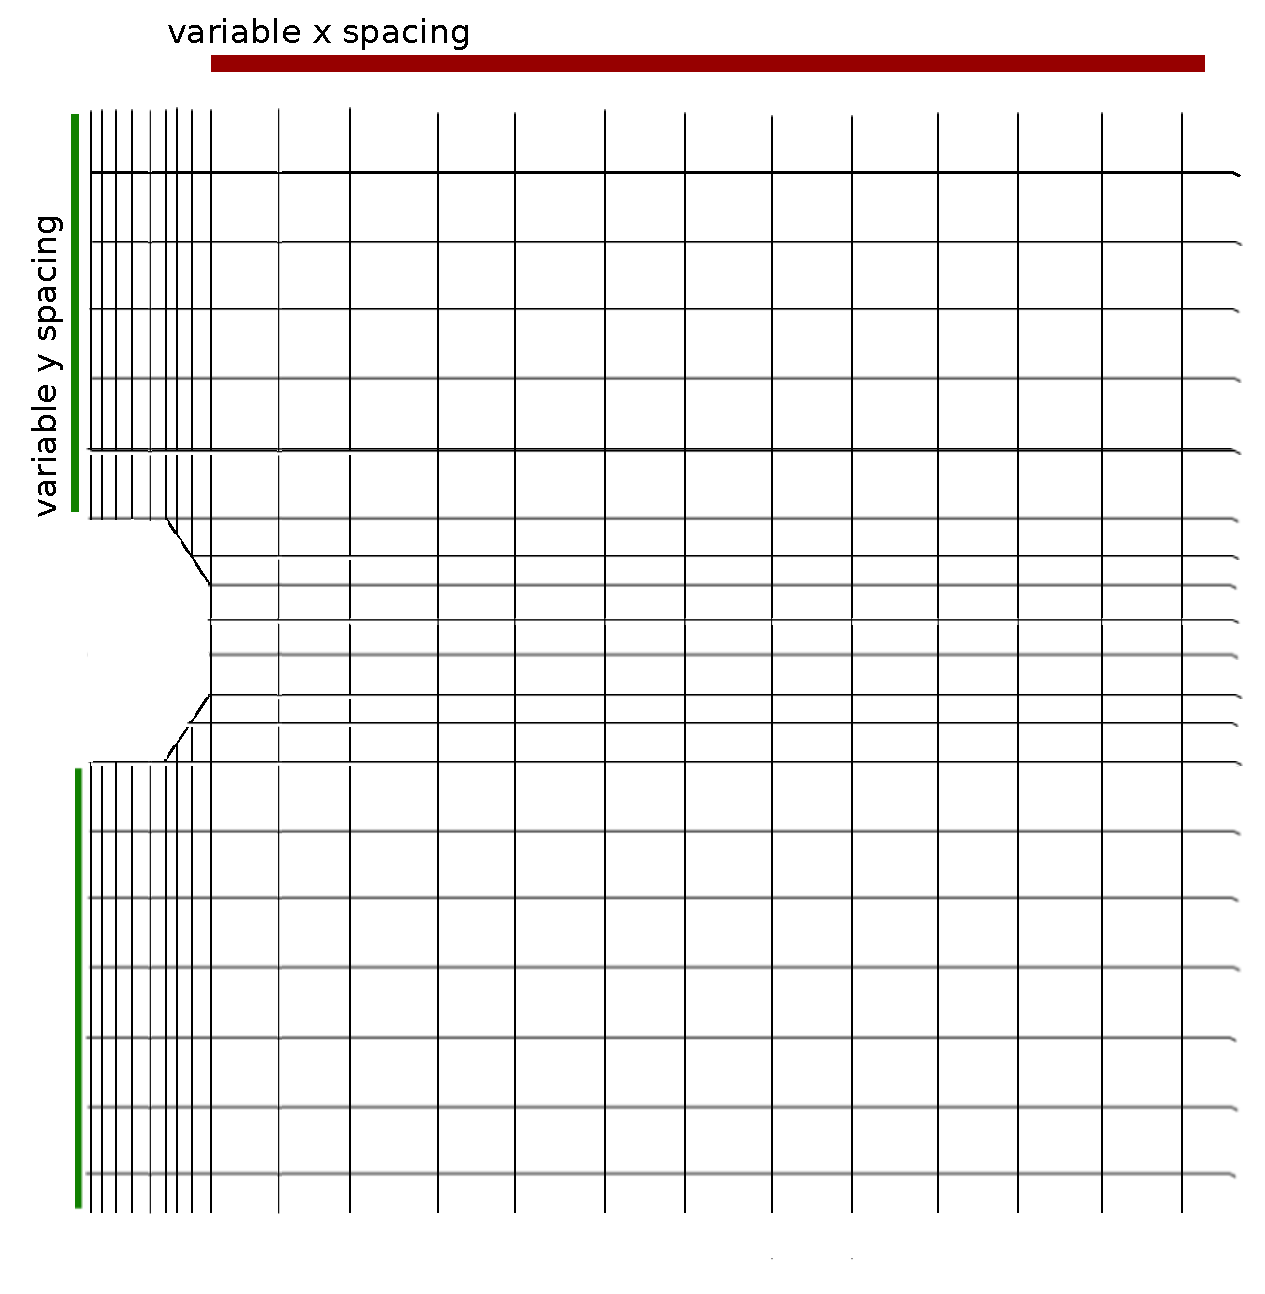
\includegraphics[height=10cm]{./chapters/litrev/sindageom.eps}
  \end{center}
  \caption[A schematic of the \gls{SINDAG} geometry.]{The geometry of the 
    \gls{SINDAG} thermal model can be adjusted in two dimensions, 
  altering the tunnel spacing and the vertical distance from the aquifer.}
  \label{fig:sindageom}
\end{figure}

The \gls{SINDAG} lumped capacitance solver solves a thermal circuit, for which 
connecting nodes may be of four types corresponding to the four modes of heat 
transfer. Nodes, treated as resistors, are connected by conduction, convection, radiation, and mass 
flow heat transfer links. As discussed in Section \ref{sec:lumpedparam}, these 
are represented by

\begin{align}
  R_{cond} &= \frac{L}{K_{th} A}\\
  R_{conv} &= \frac{1}{h A}\\
  R_{mf}  &= \frac{1}{\dot{m}c_p}\\
  R_{rad}  &= \frac{1}{\sigma F_{ij}A\left[ T_i + T_A + T_j + T_A 
  \right]\left[(T_i+T_A)^2+(T_j+T_A)^2\right]}
  \intertext{where}
  K_{th}&= ~~\mbox{thermal conductivity}[W\cdot m^{-1}\cdot K^{-1}]\nonumber\\
  A&= ~~\mbox{area} [m^2]\nonumber\\
  c_p&=~~\mbox{specific heat capacity} [J\cdot K^{-1}]\nonumber  \\
  h&= ~~\mbox{heat transfer coefficient}[W\cdot m^{-1} \cdot K^{-1}\nonumber \\
  \dot{m}&= ~~\mbox{mass transfer rate}[kg\cdot s^{-1}]\nonumber \\
  T_i&= ~~\mbox{lump temperature} [^{\circ}C] \nonumber\\
  T_A&= ~~\mbox{absolute temperature} [^{\circ}C] \nonumber\\
  F_{ij}&= ~~\mbox{radiation interchange factor} [-] .\nonumber
\end{align}

With these representations of thermal resistance, a lumped parameter model will 
require an analysis that determines the appropriate length scale for the lumped 
parameter approximation.

Given one or more heat constraints, the \gls{ANL}  model  optimizes 
spatial waste loading in order to meet those constraints with maximal waste 
loading. For example, given a thermal limit at the edge of the waste package, the 
model utilizes the \gls{SINDAG} solver to determine the two 
dimensional heat evolution of the repository as a result of a given waste package 
composition for various drift spacings and arrives at an ideal drift spacing by 
iteration.


\subsection{LLNL MathCAD Model}
\label{sec:llnl_background}

% LLNL
\subsection{Analytical Model Background}
\begin{frame}[ctb!]
\frametitle{Analytical Model : Background}
The analytical  model
\begin{itemize} 
  \item was created at LLNL (H. Greenberg, J. Blink, et. al) \cite{hardin_generic_2011, sutton_investigations_2011, 
greenberg_application_2012}
  \item employs an analytic model from Carslaw and Jaeger \cite{carslaw_conduction_1959} 
  \item is implemented in MathCAD \cite{ptc_mathcad_2010}
  \item seeks to inform heat limited waste capacity calculations for 
    \begin{itemize}
      \item arbitrary geology 
      \item arbitrary waste package loading densities
      \item arbitrary homogeneous decay heat source
    \end{itemize}
\end{itemize}
\end{frame}

\begin{frame}
  \frametitle{Analytical Model : Geometry}
  \begin{figure}[h!]
    \begin{center}
      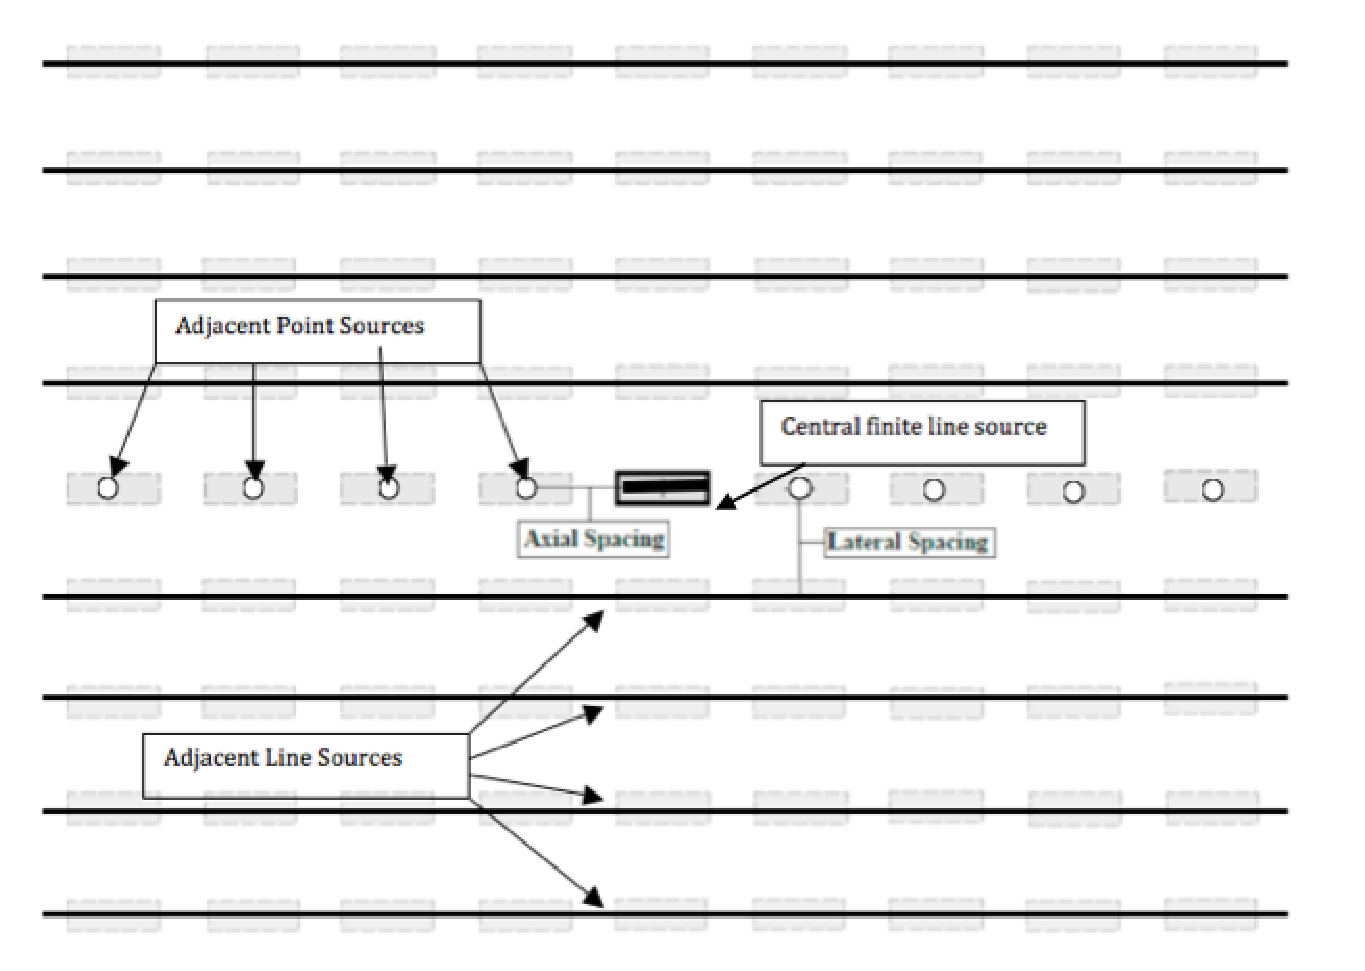
\includegraphics[width=0.7\textwidth]{./images/llnlConcept.eps}
    \caption{Vertical, horizontal, alcove, and borehole emplacement layouts can 
    be represented by a line of point sources and adjacent line sources 
    \cite{sutton_investigations_2011}.}
    \label{fig:llnl}
    \end{center}
  \end{figure}
\end{frame}

\begin{frame}
  \frametitle{Analytical Model : Calculation Method}
    LLNL's model is a MathCAD solution of the transient homogeneous 
    conduction equation,
    \begin{align}
      \nabla^2T  = \frac{1}{\alpha}\frac{\partial T}{\partial t},
      \label{condGl}
    \end{align}
    in which superimposed point and line source solutions approximate the repository 
    layout.
\end{frame}

\begin{frame}[ctb!]
\frametitle{Analytical Model : Calculation Method}
The model consists of two conceptual regions, an external region representing 
the host rock and an internal region representing the waste form, package, and 
buffer Engineered Barrier System within the disposal tunnel wall.   
\begin{itemize}
  \item Since the thermal mass of the EBS is small in comparison to the thermal 
    mass of the host rock, the internal region may be treated as quasi-steady 
    state.
  \item The transient state of the temperature at the calculation radius is 
    found with a convolution of the transient external solution with the steady 
    state internal solution.
  \item The internal and external regions are \textbf{approximated} to be a 
    single homogeneous medium.
  \item The process is then iterated with a one year resolution in order to 
    arrive at a temperature evolution over the lifetime of the repository. 
\end{itemize}
\end{frame}


\begin{frame}[ctb!]
\frametitle{Analytical Model : Calculation Method}
\begin{minipage}{0.3\textwidth}
\begin{figure}[h!]
  \begin{center}
    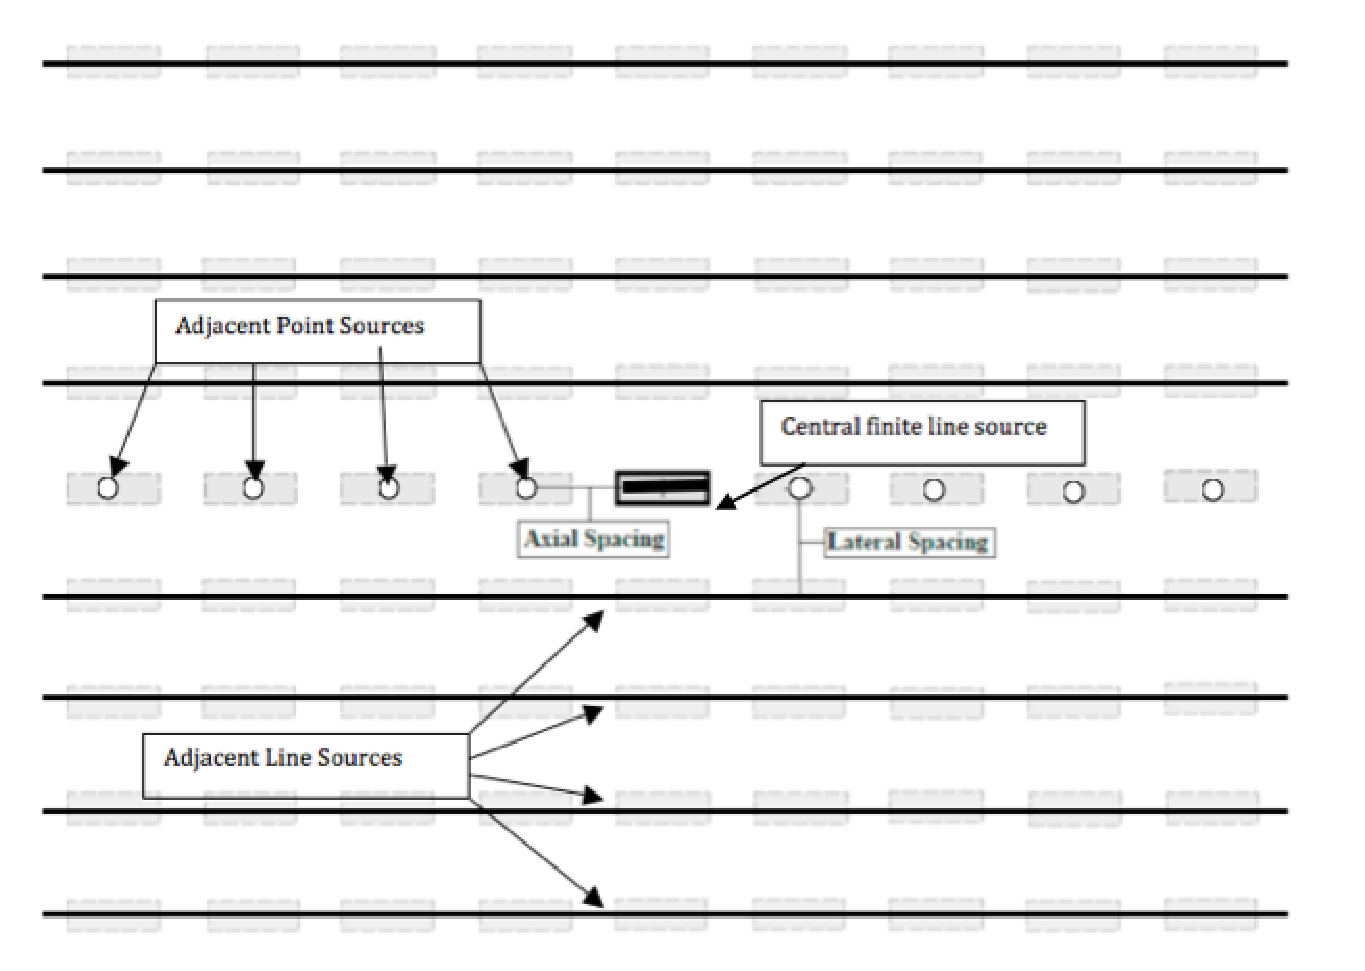
\includegraphics[width=\textwidth]{./images/llnlConcept.eps}
  \end{center}
  \caption{The central package is represented by a finite line source
  \cite{sutton_investigations_2011}.}
  \label{fig:llnl}
\end{figure}
\end{minipage}
\hspace{0.01mm}
\begin{minipage}{0.6\textwidth}
The geometric layout of the analytic LLNL model in Figure \ref{fig:llnl} 
shows  that the central package is represented by the finite line solution
\footnotesize{
\begin{align}
  T_{line}&(t,x,y,z) = \nonumber\\
  &\frac{1}{8\pi K_{th}} 
  \bigintsss_0^t\!\frac{q_L(t')}{t-t'}e^{ \frac{-\left(x^2 + z^2\right)}{4\alpha 
  (t-t')} }\nonumber\\ &\cdot\left[ \erf{\left[ \frac{1}{2} \frac{\left( y + 
  \frac{L}{2} \right)}{\sqrt{\alpha(t-t')}}  \right]} - \erf{\left[ \frac{1}{2} 
  \frac{\left( y - \frac{L}{2} \right)}{\sqrt{\alpha(t-t')}}  \right]} 
  \right]\,\mathrm{dt'}.
  \label{line}
\end{align}
}
\end{minipage}
\end{frame}

\begin{frame}[ctb!]
\frametitle{Analytical Model : Calculation Method}
\begin{minipage}{0.3\textwidth}
\begin{figure}[h!]
  \begin{center}
    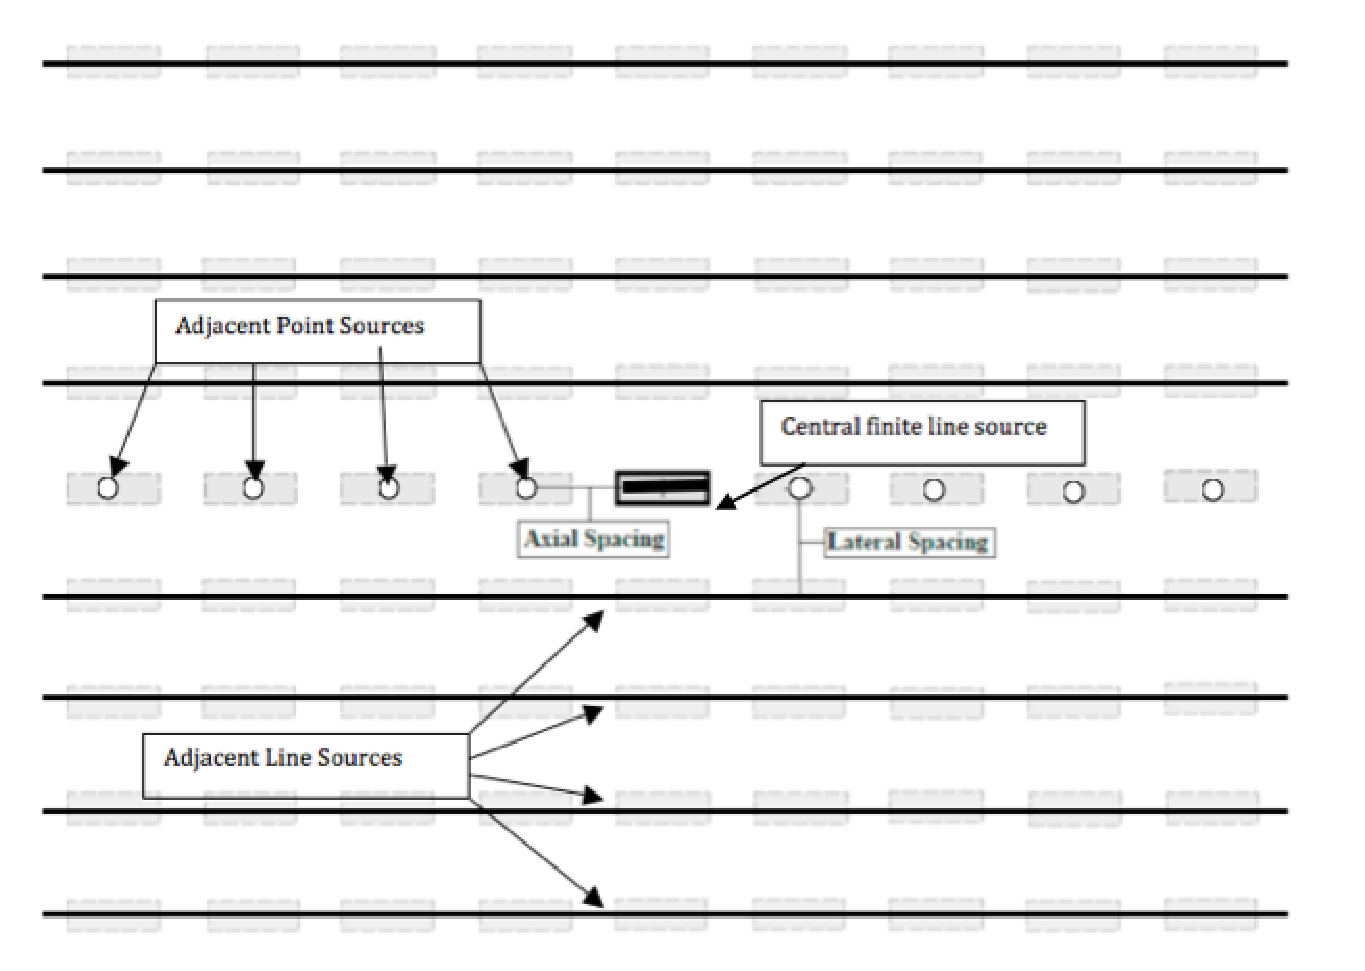
\includegraphics[width=\textwidth]{./images/llnlConcept.eps}
  \end{center}
  \caption{Adjacent packages are represented as point sources
  \cite{sutton_investigations_2011}.}
  \label{fig:llnl}
\end{figure}
\end{minipage}
\hspace{0.1mm}
\begin{minipage}{0.6\textwidth}
 Adjacent packages within the central tunnel are represented by the point source 
 solution,
 \footnotesize{
  \begin{align}
    T_{point}(t,r) &= \frac{1}{8K_{th}\sqrt{\alpha}\pi^{\frac{3}{2}}}\nonumber\\
     &\bigintsss_0^{t}\!\frac{q(t')}{(t-t')^{\frac{3}{2}}}e^{\frac{-r^2}{4\alpha(t-t')}}\,\mathrm{dt'}.
    \label{point}
  \end{align}
  }
  \end{minipage}
\end{frame}


\begin{frame}[ctb!]
\frametitle{Analytical Model : Calculation Method}
\begin{minipage}{0.3\textwidth}
\begin{figure}[h!]
  \begin{center}
    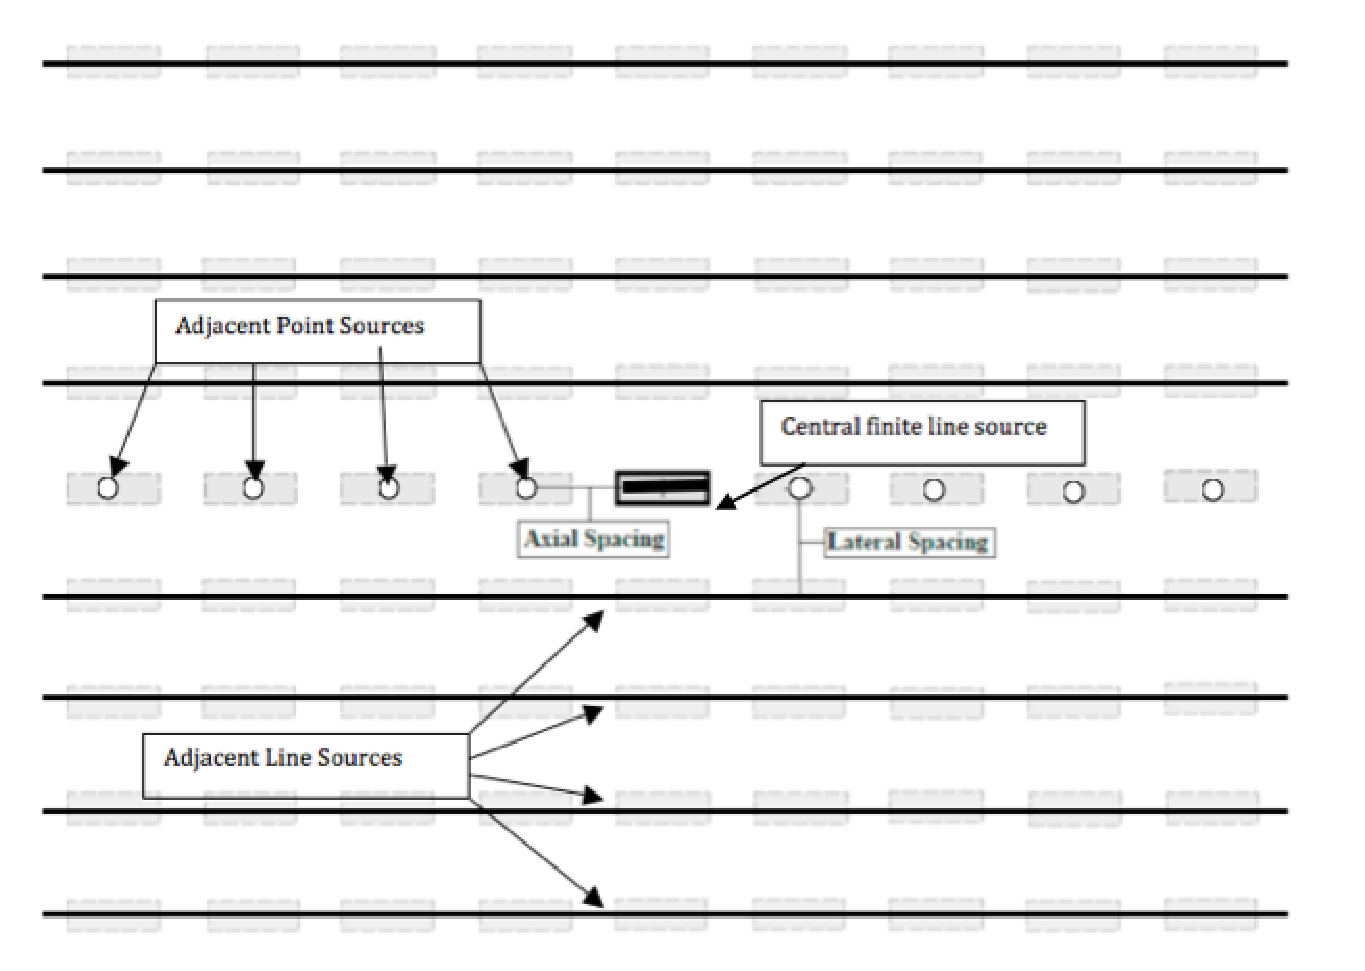
\includegraphics[width=\textwidth]{./images/llnlConcept.eps}
  \end{center}
  \caption{The non-central disposal tunnels are represented as infinite line sources
  \cite{sutton_investigations_2011}.}
  \label{fig:llnl}
\end{figure}
\end{minipage}
\hspace{0.1mm}
\begin{minipage}{0.6\textwidth}
Adjacent disposal tunnels are represented by the infinite line source solution,
\footnotesize{
\begin{align}
  T_{\infty line}(t,x,z) &= \frac{1}{4\pi K_{th}} 
  \bigintsss_0^t\frac{q_L(t')}{t-t'}e^{ \frac{-\left(x^2 + z^2\right)}{4\alpha 
  (t-t')} }
  \label{infline}
  \intertext{in infinite homogeneous media, where}
  \alpha &= ~~\mbox{thermal diffusivity } [m^2\cdot s^{-1}]\nonumber\\
  q(t) &= ~~\mbox{point heat source} [W]\nonumber\\
  \intertext{and}
  q_L(t) &= ~~\mbox{linear heat source} [W\cdot m^{-1}]\nonumber
\end{align}
}
Superimposed point and line source solutions allow for a notion of the 
repository layout to be modeled in the host rock.
\end{minipage}
\end{frame}




\subsection{Yucca Mountain Layout Analyses}

The repository layout has a significant influence on its heat transfer 
properties.  Waste package spacing in drifts, boreholes, or alcoves, tunnel
spacing, and multiple gallery level designs all define available 
heat loading.  For example, in the \gls{YMR}, a variety of parameters have been 
shown to affect the potential repository waste loading density. 

The \gls{YMR} statutory limit of once-through, thermal PWR waste was 70,000 
\gls{MTHM} of waste.  That is to say, the statutory line load limit is approximately 1.04 tonnes/m
for 67km of planned emplacement tunnels (with 81 meters between drifts). The
Office of Civilian Radioactive Waste Management Science and Engineering Report
gives this basic ``statutory limit'', but suggests an inherent design
flexibility that could allow for expansion. Multiple efforts have adjusted 
various repository layout parameters in order to develop expanded capacity 
models of the \gls{YMR}. Some of these efforts are detailed in Table 
\ref{tab:footprint}.

\begin{table}[h!]
  \centering
      \footnotesize{
      \begin{tabularx}{\textwidth}{|X|c|c|X|}
          \multicolumn{4}{c}{\textbf{Yucca Mountain Footprint Expansion Calculations}}\\
          \hline
          Author&Max. Capacity&Footprint&Details\\
          &$tonnes$&$km^2$&\\
          \hline
          &&&\\
          OCRWM&$70,000$&$4.65$&``statutory case''\\
          &$97,000$&$6$&``full inventory case''\\
          &$119,000$&$~7$&``additional case''\\
          \hline
          &&&\\
          Yim, M.S.&$75,187$&$4.6$&SRTA code\\
          &$76,493$&$4.6$&STI method\\
          &$95,970$&$4.6$&$63$m drift spacing\\
          &$82,110$&$4.6$&75 yrs. cooling\\
          \hline
          &&&\\
          Nicholson, M.&$103,600$&$4.6$&drift spacing\\
          \hline
          &&&\\
          EPRI&&&\\
          &$63,000$&$6.5$&Base Case CSNF\\
          option 1&$126,000$&$13$&expanded footprint\\
          option 2&$189,000$&$6.5$&multi-level design\\
          option 3&$189,000$&$6.5$&grouped drifts\\
          options 2+3&$252,000$&$6.5$&hybrid\\
          options 1+(2or3) &$378,000$&$13$&hybrid\\
          options 1+2+3 &$567,000$&$13$&hybrid\\
          \hline
        \end{tabularx}
        \caption[Yucca Mountain footprint expansion calculations.]{Various analyses based on heat 
        load limited repository designs have resulted in footprint expansion calculations of the 
        YMR.} 
        \label{tab:footprint}
        }
      \end{table}
 

This inherent flexibility can come from an increase in the areal extent of the 
repository footprint, the density of drifts, or vertical expansion. The  ``full inventory'' Yucca
Mountain design alternative gives a maximum repository capacity of 97,000
tonnes. In addition, the current design for the repository has flexibility for
``additional repository capacity'' which would give a 119,000 tonne capacity at
1.04 tonnes/m.\cite{doe_yucca_2002} 

In addition to variable drift spacing, other modifications to repository layout
have had promising results in terms of heat-limited repository capacity. The
Electric Power Research Institute (EPRI) in their Room at the Mountain study
found that with redesign of the repository an increased capacity of at least
$400\%$ (295 kilotonnes once-through SNF) and up to $900\%$ (663 kilotonnes) could be
expected to be achieved. Proposed design changes include decreased spacing
between drifts, a larger areal footprint, vertical expansion into second and
third levels of repository space, and hybrid solutions involving combinations
of these ideas. In particular, EPRI suggests either an expansion of the
footprint with redesign of the current line load design plan or a
multi-level plan that repeats the footprint and line load design of the current
plan\cite{kessler_room_2006}.

%Specific Temperature Change analysis by Radel, Wilson, et al. find a maximum
%thermal capacity of 1.09 tonnes/m for commercial SNF (at an ELF of $49
%GWd_{th}/m$)\cite{radel_effect_2007}. 

Layout options such as age based fuel mixing also allows for decreases in drift 
spacing. In aged based fuel mixing, aged (long cool time) SNF is loaded in a 
mixture with young SNF. This age based fuel mixing has been shown to achieve a 
$48\%$ increase in the repository capacity as constrained by heat
load\cite{nicholson_thermal_2007}. This factor uses a fiducial default
footprint of $4.6 km^2$ used in the NRC TSPA.  The reported $48\%$ increase in
capacity results in total repository capacity of 103,600
tonnes\cite{williams_total_2001}.


\subsection{Other Numerical Methods}

Codes used by repository modeling efforts investigated in this review include 
finite difference codes, finite element codes, and specific temperature 
integrals.  Some efforts and their methods are listed in Table \ref{tab:heat}.


%%%%%%%%%%%%%%%%%%%%%%%%%%%%%%%%%%%%%%%%%%%%%%%% 
%%%%% Heat Load Computational Models Table %%%%% 
%%%%%%%%%%%%%%%%%%%%%%%%%%%%%%%%%%%%%%%%%%%%%%%% 

 \begin{table}[h!]
    \centering
    \footnotesize{
    \begin{tabularx}{\textwidth}{|X|c|c|X|}
      \multicolumn{4}{c}{\textbf{Models of Heat Load for Various Geologic Media}}\\
      \hline
      Source & Nation & Geology & Methodology \\  
      (Who) & (Where) & (What) & (How) \\  
      \hline
      Enresa \cite{von_lensa_red-impact_2008}           & Spain       & Granite       &  CODE\_BRIGHT 3D Finite Element \\ 
      NRI   \cite{von_lensa_red-impact_2008}            & Czech Rep.  & Granite       &  Specific Temperature Integral   \\
      ANDRA \cite{andra_granite:_2005}                  & France      & Granite       &  3D Finite Element CGM code   \\
      SKB \cite{ab_long-term_2006}                      & Sweden      & metagranite   &  1D-3D Site  Descriptive Models \\
      SCK$\cdot$CEN   \cite{von_lensa_red-impact_2008}  & Belgium     & Clay          &  Specific Temperature Integral   \\ 
      ANDRA \cite{andra_argile:_2005}                   & France      & Argile Clay   &  3D Finite Element CGM code   \\
      NAGRA \cite{johnson_project_2002, johnson_calculations_2002}  & Switzerland  & Opalinus Clay &  3D Finite Element CGM code \\
      GRS \cite{von_lensa_red-impact_2008}              & Germany     & Salt          &  HEATING (3D finite difference)   \\ 
      NCSU(Li)   \cite{li_examining_2007}               & USA         & Yucca Tuff    &  Specific Temperature Integral \\        
      NCSU(Nicholson) \cite{nicholson_thermal_2007}     & USA         & Yucca Tuff    &  COSMOL 3D Finite Element\\
      Radel \& Wilson \cite{radel_repository_2007}      & USA         & Yucca Tuff    &  Specific Temperature Change \\ 
      \hline
    \end{tabularx}
    \caption[International heat transport modeling methods in various geologic host media.]{Methods by which to calculate heat 
    load are independent of geology. Maximum heat load constraints, however, vary among host formations. }
    \label{tab:heat}
    }
  \end{table}


%%%%%%%%%%%%%%%%%%%%%%%%%%%%%%%%%%%%%%



